% Seminarul 9: Învățare automată pentru serii de timp
% Serii de timp -- Programele de licență Informatică economică și Cibernetică economică, Academia de Studii Economice din București
% GENERAT de latex/build_seminar9.py -- modificați generatorul, nu acest fișier.
% Implicit versiunea pentru studenți; versiunea profesorului este wrapper-ul *_solutions.tex.
\makeatletter\@ifundefined{ifsolutions}{\expandafter\newif\csname ifsolutions\endcsname}{}\makeatother

\newcommand{\coursename}{Serii de timp}
\def\tsalang{ro}
% Preambul comun TSA -- Serii de timp / Time Series Analysis (Beamer, 16:9)
% Același design ca MFM și SFM (preluat din SFM, 5 octombrie 2026). Înainte de % Preambul comun TSA -- Serii de timp / Time Series Analysis (Beamer, 16:9)
% Același design ca MFM și SFM (preluat din SFM, 5 octombrie 2026). Înainte de % Preambul comun TSA -- Serii de timp / Time Series Analysis (Beamer, 16:9)
% Același design ca MFM și SFM (preluat din SFM, 5 octombrie 2026). Înainte de \input{../../latex/preamble} se definește
%   \newcommand{\coursename}{Time Series Analysis}      (EN)
%   \newcommand{\coursename}{Serii de timp}       (RO)  și  \def\tsalang{ro}
% Fișierele .tex se află în EN/Courses, EN/Seminars, RO/Cursuri, RO/Seminarii (două niveluri sub rădăcină).
% Deck-urile sînt generate de latex/build_chapterN.py / build_seminarN.py (vezi latex/tsa_build.py).

\documentclass[9pt, aspectratio=169, t]{beamer}
\providecommand{\coursename}{Time Series Analysis}

% Ensure content fits on slides
\setbeamersize{text margin left=8mm, text margin right=8mm}
% Smaller institute font (title page)
\setbeamerfont{institute}{size=\footnotesize}

%=============================================================================
% THEME AND STYLE CONFIGURATION
%=============================================================================
\usetheme{default}
% Using default theme for clean header/footer control

% Color Palette (matching Redispatch PDF)
\definecolor{MainBlue}{RGB}{26, 58, 110}
\definecolor{AccentBlue}{RGB}{26, 58, 110}
\definecolor{IDAred}{RGB}{205, 0, 0}
\definecolor{DarkGray}{RGB}{51, 51, 51}
\definecolor{MediumGray}{RGB}{128, 128, 128}
\definecolor{LightGray}{RGB}{248, 248, 248}
\definecolor{VeryLightGray}{RGB}{235, 235, 235}
\definecolor{KeynoteGray}{RGB}{218, 218, 218}
\definecolor{SectionGray}{RGB}{120, 120, 120}
\definecolor{FooterGray}{RGB}{100, 100, 100}
\definecolor{Crimson}{RGB}{220, 53, 69}
\definecolor{Forest}{RGB}{46, 125, 50}
\definecolor{Amber}{RGB}{181, 133, 63}
\definecolor{Orange}{RGB}{230, 126, 34}
\definecolor{Purple}{RGB}{142, 68, 173}

% Gradient background (exact Keynote 315° gradient: white to RGB 218,218,218)
\setbeamertemplate{background}{%
    \begin{tikzpicture}[remember picture, overlay]
        \shade[shading=axis, shading angle=315,
        top color=white, bottom color=KeynoteGray]
        (current page.south west) rectangle (current page.north east);
    \end{tikzpicture}%
}
% Fallback solid color for compatibility
\setbeamercolor{background canvas}{bg=}

\setbeamercolor{palette primary}{bg=MainBlue, fg=white}
\setbeamercolor{palette secondary}{bg=MainBlue!85, fg=white}
\setbeamercolor{palette tertiary}{bg=MainBlue!70, fg=white}
\setbeamercolor{structure}{fg=MainBlue}
\setbeamercolor{title}{fg=IDAred}
\setbeamercolor{frametitle}{fg=IDAred, bg=}
\setbeamercolor{block title}{bg=MainBlue, fg=white}
\setbeamercolor{block body}{bg=VeryLightGray, fg=DarkGray}
\setbeamercolor{block title alerted}{bg=Crimson, fg=white}
\setbeamercolor{block body alerted}{bg=Crimson!8, fg=DarkGray}
\setbeamercolor{block title example}{bg=Forest, fg=white}
\setbeamercolor{block body example}{bg=Forest!8, fg=DarkGray}
\setbeamercolor{item}{fg=MainBlue}

% Footer colors (override Madrid theme blue)
\setbeamercolor{author in head/foot}{fg=FooterGray, bg=}
\setbeamercolor{title in head/foot}{fg=FooterGray, bg=}
\setbeamercolor{date in head/foot}{fg=FooterGray, bg=}
\setbeamercolor{section in head/foot}{fg=FooterGray, bg=}
\setbeamercolor{subsection in head/foot}{fg=FooterGray, bg=}

% Bullet styles (apply everywhere including blocks)
\setbeamertemplate{itemize item}{\color{MainBlue}$\boxdot$}
\setbeamertemplate{itemize subitem}{\color{MainBlue}$\blacktriangleright$}
\setbeamertemplate{itemize subsubitem}{\color{MainBlue}\tiny$\bullet$}
\setbeamertemplate{itemize/enumerate body begin}{\normalsize}
\setbeamertemplate{itemize/enumerate subbody begin}{\normalsize}

% Item spacing - compact style
\setlength{\leftmargini}{10pt}       % Level 1: minimal indent
\setlength{\leftmarginii}{10pt}      % Level 2: minimal additional indent
% Compact list spacing (zero extra space before/after lists in blocks)
\makeatletter
\def\@listi{\leftmargin\leftmargini \topsep 0pt \parsep 0pt \itemsep 0pt}
\def\@listii{\leftmargin\leftmarginii \topsep 0pt \parsep 0pt \itemsep 0pt}
\makeatother

\setbeamertemplate{navigation symbols}{}

%=============================================================================
% CUSTOM HEADLINE
%=============================================================================
\setbeamertemplate{headline}{%
    \vskip10pt%
    \hbox to \paperwidth{%
        \hskip0.5cm%
        {\small\color{FooterGray}\renewcommand{\hyperlink}[2]{##2}\insertsectionhead}%
        \hfill%
        \textcolor{FooterGray}{\small\insertframenumber}%
        \hskip0.5cm%
    }%
    \vskip4pt%
    {\color{FooterGray}\hrule height 0.4pt}%
}

%=============================================================================
% CUSTOM FOOTER
%=============================================================================
\usepackage{fontawesome5}

\setbeamertemplate{footline}{%
    {\color{FooterGray}\hrule height 0.4pt}%
    \vskip4pt%
    \hbox to \paperwidth{%
        \hskip0.5cm%
        \textcolor{FooterGray}{\small\coursename}%
        \hfill%
        \raisebox{-0.1em}{%
            \begin{tikzpicture}[x=0.08em, y=0.08em, line width=0.4pt]
                \draw[FooterGray] (0,3) -- (1,4) -- (2,3.5) -- (3,5) -- (4,4) -- (5,6) -- (6,5.5) -- (7,4) -- (8,5) -- (9,7) -- (10,6) -- (11,5) -- (12,6.5) -- (13,8) -- (14,7) -- (15,6) -- (16,7.5) -- (17,9) -- (18,8) -- (19,7) -- (20,8.5) -- (21,10) -- (22,9) -- (23,8) -- (24,9.5);
            \end{tikzpicture}%
        }%
        \hskip0.5cm%
    }%
    \vskip6pt%
}

%=============================================================================
% PACKAGES
%=============================================================================
\usepackage[utf8]{inputenc}
\DeclareUnicodeCharacter{03B1}{\ensuremath{\alpha}}
\usepackage[T1]{fontenc}
\usepackage{amsmath, amssymb, amsthm}
\usepackage{mathtools}
\usepackage{bm}
\usepackage{tikz}
\usetikzlibrary{arrows.meta, positioning, shapes, calc, decorations.pathreplacing, shadings}
\usepackage{booktabs}
\usepackage{multirow}
\usepackage{array}
\usepackage{graphicx}
\usepackage{animate}
\usepackage{hyperref}
\usepackage{colortbl}
\usepackage{listings}
\lstset{language=Python, basicstyle=\ttfamily\scriptsize, keywordstyle=\color{MainBlue}\bfseries,
  commentstyle=\color{Forest}, stringstyle=\color{Crimson}, breaklines=true,
  frame=none, backgroundcolor=\color{VeryLightGray}, xleftmargin=2mm}
\hypersetup{colorlinks=true, linkcolor=MainBlue, urlcolor=MainBlue}
\graphicspath{{../../logos/}{../../charts/}{../../photos/}}
\usepackage{xcolor}
\hfuzz=2pt  % Suppress tiny overfull warnings (<2pt)
\vfuzz=2pt  % Suppress tiny vertical overfull warnings (<2pt)
% \mathrm in the sans-serif family of the slides (beamer resets \mathrm to the serif family at \begin{document};
% this hook runs after beamer's, so WN, Var, RMSE, ... in formulas match the surrounding text)
% Bold vectors and matrices in the same sans-serif family: \mathbf{A} in sans bold (beamer's own \mathbf came out in
% medium weight), and the bold upright Greek capitals of \boldsymbol / \bm (\bSigma, \bPhi, \boldsymbol{\Theta}) in
% cmss bold: bm.sty fixes its "boldoperators" font when it is loaded (serif cmbx), before beamer switches the
% operators to cmss, so it is reset here.
\AtBeginDocument{%
  \SetMathAlphabet{\mathrm}{normal}{\encodingdefault}{\sfdefault}{\mddefault}{n}%
  \SetMathAlphabet{\mathrm}{bold}{\encodingdefault}{\sfdefault}{bx}{n}%
  \SetMathAlphabet{\mathbf}{normal}{\encodingdefault}{\sfdefault}{bx}{n}%
  \SetMathAlphabet{\mathbf}{bold}{\encodingdefault}{\sfdefault}{bx}{n}%
  \SetSymbolFont{boldoperators}{normal}{OT1}{cmss}{bx}{n}%
  \SetSymbolFont{boldoperators}{bold}{OT1}{cmss}{bx}{n}}

%=============================================================================
% QUANTLET COMMANDS
%   \quantlet{<displayed name>}{<url>}       (generic, compatible with the older TSA decks)
%   \tsaquantlet{Ch_05}{TSA_ch5_garch}       -> https://github.com/danpele/Time-Series-Analysis/tree/main/Quantlets/Ch_05/TSA_ch5_garch
%   \qlurl{<folder>} is defined per chapter by the generator (Quantlets/Ch_NN/<folder>)
%=============================================================================
\newcommand{\tsarepo}{https://github.com/danpele/Time-Series-Analysis}
\newcommand{\tsaqlbase}{https://github.com/danpele/Time-Series-Analysis/tree/main/Quantlets}
\newcommand{\quantlet}[2]{%
    \hfill\href{#2}{%
        \raisebox{-0.15em}{
\includegraphics[height=0.7em]{ql_logo.png}}%
        \textcolor{MainBlue}{\tiny\ #1}%
    }%
}
\newcommand{\tsaquantlet}[2]{\quantlet{\detokenize{#2}}{\tsaqlbase/#1/#2}}

%=============================================================================
% NOTEBOOKS (Google Colab)
%   \colaburl{notebooks/EN/chapter5_seminar_notebook.ipynb} -> the Colab link of a file in the TSA repo
%   \nb: the chapter notebook (each seminar deck redefines it with \renewcommand)
%=============================================================================
\newcommand{\colaburl}[1]{https://colab.research.google.com/github/danpele/Time-Series-Analysis/blob/main/#1}
\newcommand{\nb}{https://colab.research.google.com/github/danpele/Time-Series-Analysis/tree/main/notebooks/EN}
\newcommand{\nbname}{notebooks/EN}

%=============================================================================
% SLIDE HELPERS (used by the generators; the same as in MFM)
%=============================================================================
% local font size for list bodies (the preamble forces \normalsize)
\newcommand{\itemsize}[1]{\setbeamertemplate{itemize/enumerate body begin}{#1}\setbeamertemplate{itemize/enumerate subbody begin}{#1}}
\newcommand{\intitle}[1]{{\hypersetup{urlcolor=white}#1}}   % white links inside coloured title bars
\newcommand{\imgcap}[1]{{\scriptsize #1}\\[0.5mm]}          % caption under a photo
\newcommand{\imgcredit}[2]{{\tiny\color{FooterGray}\href{#1}{#2}}}   % image credit: source URL, author/licence
\newcommand{\aiprompt}[1]{{\ttfamily\color{MainBlue}#1}}     % a prompt to an AI assistant

%=============================================================================
% SEMINARS: student version by default; the instructor wrapper *_solutions.tex sets \solutionstrue
%=============================================================================
\makeatletter\@ifundefined{ifsolutions}{\expandafter\newif\csname ifsolutions\endcsname}{}\makeatother
\newcommand{\solonly}[1]{\ifsolutions #1\fi}
\newcommand{\propsub}{\ifsolutions\else\framesubtitle{\ifdefined\tsalang Rezolvarea se discută la seminar\else Solution discussed in class\fi}\fi}

%=============================================================================
% APPENDIX AND CHAPTER LINKS (latex/appendix_links.py writes the calls; it also re-declares these
% macros before \begin{document}, so the decks compile with or without this preamble block)
%=============================================================================
\providecommand{\tsaapplink}[3]{\hypertarget{#2}{}\hyperlink{#1}{\beamergotobutton{#3}}}
\providecommand{\tsaappback}[2]{\begin{tikzpicture}[remember picture,overlay]\node[anchor=south east] at ([xshift=-3mm,yshift=7mm]current page.south east){\hyperlink{#1}{\beamerreturnbutton{#2}}};\end{tikzpicture}}
\providecommand{\tsachlink}[2]{\href{#1}{#2}}
\providecommand{\tsachlinkt}[2]{\href{#1}{\usebeamercolor[fg]{frametitle}#2}}

%=============================================================================
% QUANTINAR COMMAND: link către un curs Quantinar (subiecte avansate)
%=============================================================================
\newcommand{\quantinar}[2]{%
    \href{#2}{%
        \raisebox{-0.15em}{
\includegraphics[height=0.8em]{qr_logo.png}}%
        \textcolor{MainBlue}{\scriptsize\ #1}%
    }%
}

%=============================================================================
% CUSTOM TITLE PAGE
%=============================================================================
\defbeamertemplate*{title page}{hybrid}[1][]
{
    \vspace{0.2cm}
    % Logos row - top header (with clickable links)
    \begin{center}
        \href{https://www.ase.ro}{
\includegraphics[height=1.0cm]{ase_logo.png}}\hspace{0.3cm}%
        \href{https://theida.net}{
\includegraphics[height=1.0cm]{ida_logo.png}}\hspace{0.3cm}%
        \href{https://blockchain-research-center.com}{
\includegraphics[height=1.0cm]{brc_logo.png}}\hspace{0.3cm}%
        \href{https://www.ai4efin.ase.ro}{
\includegraphics[height=1.0cm]{ai4efin_logo.png}}\hspace{0.3cm}%
        \href{https://ipe.ro/new}{
\includegraphics[height=1.0cm]{acad_logo.png}}\hspace{0.3cm}%
        \href{https://www.digital-finance-msca.com}{
\includegraphics[height=1.0cm]{msca_logo.png}}%
    \end{center}

    \vspace{0.6cm}

    % Main title with Q logos on sides (with clickable links)
    \begin{center}
        \begin{minipage}{0.1\textwidth}
            \centering
            \href{https://quantlet.com}{
\includegraphics[height=1.1cm]{ql_logo.png}}
        \end{minipage}%
        \begin{minipage}{0.78\textwidth}
            \centering
            {\LARGE\bfseries\usebeamercolor[fg]{title}\inserttitle}

            \vspace{0.3cm}

            {\usebeamerfont{subtitle}\usebeamercolor[fg]{title}\insertsubtitle}
        \end{minipage}%
        \begin{minipage}{0.1\textwidth}
            \centering
            \href{https://quantinar.com}{
\includegraphics[height=1.1cm]{qr_logo.png}}
        \end{minipage}
    \end{center}

    \vspace{0.6cm}

    % Authors (left aligned)
    \hspace{0.5cm}{\usebeamerfont{author}\insertauthor}

    \vspace{0.3cm}

    % Institute/Affiliations (left aligned)
    \hspace{0.5cm}\begin{minipage}[t]{0.9\textwidth}
        \raggedright\small\insertinstitute
    \end{minipage}
}

%=============================================================================
% THEOREM ENVIRONMENTS
%=============================================================================
\theoremstyle{definition}
\setbeamertemplate{theorems}[numbered]
\ifdefined\tsalang
\newtheorem{defn}{Definiție}
\newtheorem{thm}{Teoremă}
\newtheorem{prop}{Propoziție}
\newtheorem{rmk}{Observație}
\else
\newtheorem{defn}{Definition}
\newtheorem{thm}{Theorem}
\newtheorem{prop}{Proposition}
\newtheorem{rmk}{Remark}
\fi

%=============================================================================
% CENTRED MINIPAGE (no extra vertical space)
%=============================================================================
\newenvironment{cminipage}[1]{%
    \par\noindent\hfill\begin{minipage}{#1}\ignorespaces
}{%
    \end{minipage}\hfill\null\par
}

%=============================================================================
% CUSTOM COMMANDS
%=============================================================================
\newcommand{\E}{\mathbb{E}}
\newcommand{\Var}{\text{Var}}
\newcommand{\Cov}{\text{Cov}}
\newcommand{\Corr}{\text{Corr}}
\newcommand{\R}{\mathbb{R}}
\newcommand{\N}{\mathbb{N}}
\newcommand{\Z}{\mathbb{Z}}
\newcommand{\B}{\mathbf{B}}
\newcommand{\imark}{\textcolor{MainBlue}{\textbullet}}
\newcommand{\RMSE}{\text{RMSE}}
\newcommand{\MAE}{\text{MAE}}
\newcommand{\MAPE}{\text{MAPE}}

% Boldface vector/matrix commands (VAR, VECM, state space; also used by the older TSA decks)
\newcommand{\bY}{\mathbf{Y}}
\newcommand{\bX}{\mathbf{X}}
\newcommand{\bA}{\mathbf{A}}
\newcommand{\bB}{\mathbf{B}}
\newcommand{\bepsilon}{\boldsymbol{\varepsilon}}
\newcommand{\bSigma}{\boldsymbol{\Sigma}}
\newcommand{\bPhi}{\boldsymbol{\Phi}}
\newcommand{\bGamma}{\boldsymbol{\Gamma}}
\newcommand{\bPi}{\boldsymbol{\Pi}}
\newcommand{\bc}{\mathbf{c}}
\newcommand{\balpha}{\boldsymbol{\alpha}}
\newcommand{\bbeta}{\boldsymbol{\beta}}
\newcommand{\bvarepsilon}{\boldsymbol{\varepsilon}}

% Legacy seminar marks (older TSA seminar decks)
\newcommand{\correct}{\textcolor{Forest}{\checkmark}}
\newcommand{\incorrect}{\textcolor{Crimson}{\texttimes}}
 se definește
%   \newcommand{\coursename}{Time Series Analysis}      (EN)
%   \newcommand{\coursename}{Serii de timp}       (RO)  și  \def\tsalang{ro}
% Fișierele .tex se află în EN/Courses, EN/Seminars, RO/Cursuri, RO/Seminarii (două niveluri sub rădăcină).
% Deck-urile sînt generate de latex/build_chapterN.py / build_seminarN.py (vezi latex/tsa_build.py).

\documentclass[9pt, aspectratio=169, t]{beamer}
\providecommand{\coursename}{Time Series Analysis}

% Ensure content fits on slides
\setbeamersize{text margin left=8mm, text margin right=8mm}
% Smaller institute font (title page)
\setbeamerfont{institute}{size=\footnotesize}

%=============================================================================
% THEME AND STYLE CONFIGURATION
%=============================================================================
\usetheme{default}
% Using default theme for clean header/footer control

% Color Palette (matching Redispatch PDF)
\definecolor{MainBlue}{RGB}{26, 58, 110}
\definecolor{AccentBlue}{RGB}{26, 58, 110}
\definecolor{IDAred}{RGB}{205, 0, 0}
\definecolor{DarkGray}{RGB}{51, 51, 51}
\definecolor{MediumGray}{RGB}{128, 128, 128}
\definecolor{LightGray}{RGB}{248, 248, 248}
\definecolor{VeryLightGray}{RGB}{235, 235, 235}
\definecolor{KeynoteGray}{RGB}{218, 218, 218}
\definecolor{SectionGray}{RGB}{120, 120, 120}
\definecolor{FooterGray}{RGB}{100, 100, 100}
\definecolor{Crimson}{RGB}{220, 53, 69}
\definecolor{Forest}{RGB}{46, 125, 50}
\definecolor{Amber}{RGB}{181, 133, 63}
\definecolor{Orange}{RGB}{230, 126, 34}
\definecolor{Purple}{RGB}{142, 68, 173}

% Gradient background (exact Keynote 315° gradient: white to RGB 218,218,218)
\setbeamertemplate{background}{%
    \begin{tikzpicture}[remember picture, overlay]
        \shade[shading=axis, shading angle=315,
        top color=white, bottom color=KeynoteGray]
        (current page.south west) rectangle (current page.north east);
    \end{tikzpicture}%
}
% Fallback solid color for compatibility
\setbeamercolor{background canvas}{bg=}

\setbeamercolor{palette primary}{bg=MainBlue, fg=white}
\setbeamercolor{palette secondary}{bg=MainBlue!85, fg=white}
\setbeamercolor{palette tertiary}{bg=MainBlue!70, fg=white}
\setbeamercolor{structure}{fg=MainBlue}
\setbeamercolor{title}{fg=IDAred}
\setbeamercolor{frametitle}{fg=IDAred, bg=}
\setbeamercolor{block title}{bg=MainBlue, fg=white}
\setbeamercolor{block body}{bg=VeryLightGray, fg=DarkGray}
\setbeamercolor{block title alerted}{bg=Crimson, fg=white}
\setbeamercolor{block body alerted}{bg=Crimson!8, fg=DarkGray}
\setbeamercolor{block title example}{bg=Forest, fg=white}
\setbeamercolor{block body example}{bg=Forest!8, fg=DarkGray}
\setbeamercolor{item}{fg=MainBlue}

% Footer colors (override Madrid theme blue)
\setbeamercolor{author in head/foot}{fg=FooterGray, bg=}
\setbeamercolor{title in head/foot}{fg=FooterGray, bg=}
\setbeamercolor{date in head/foot}{fg=FooterGray, bg=}
\setbeamercolor{section in head/foot}{fg=FooterGray, bg=}
\setbeamercolor{subsection in head/foot}{fg=FooterGray, bg=}

% Bullet styles (apply everywhere including blocks)
\setbeamertemplate{itemize item}{\color{MainBlue}$\boxdot$}
\setbeamertemplate{itemize subitem}{\color{MainBlue}$\blacktriangleright$}
\setbeamertemplate{itemize subsubitem}{\color{MainBlue}\tiny$\bullet$}
\setbeamertemplate{itemize/enumerate body begin}{\normalsize}
\setbeamertemplate{itemize/enumerate subbody begin}{\normalsize}

% Item spacing - compact style
\setlength{\leftmargini}{10pt}       % Level 1: minimal indent
\setlength{\leftmarginii}{10pt}      % Level 2: minimal additional indent
% Compact list spacing (zero extra space before/after lists in blocks)
\makeatletter
\def\@listi{\leftmargin\leftmargini \topsep 0pt \parsep 0pt \itemsep 0pt}
\def\@listii{\leftmargin\leftmarginii \topsep 0pt \parsep 0pt \itemsep 0pt}
\makeatother

\setbeamertemplate{navigation symbols}{}

%=============================================================================
% CUSTOM HEADLINE
%=============================================================================
\setbeamertemplate{headline}{%
    \vskip10pt%
    \hbox to \paperwidth{%
        \hskip0.5cm%
        {\small\color{FooterGray}\renewcommand{\hyperlink}[2]{##2}\insertsectionhead}%
        \hfill%
        \textcolor{FooterGray}{\small\insertframenumber}%
        \hskip0.5cm%
    }%
    \vskip4pt%
    {\color{FooterGray}\hrule height 0.4pt}%
}

%=============================================================================
% CUSTOM FOOTER
%=============================================================================
\usepackage{fontawesome5}

\setbeamertemplate{footline}{%
    {\color{FooterGray}\hrule height 0.4pt}%
    \vskip4pt%
    \hbox to \paperwidth{%
        \hskip0.5cm%
        \textcolor{FooterGray}{\small\coursename}%
        \hfill%
        \raisebox{-0.1em}{%
            \begin{tikzpicture}[x=0.08em, y=0.08em, line width=0.4pt]
                \draw[FooterGray] (0,3) -- (1,4) -- (2,3.5) -- (3,5) -- (4,4) -- (5,6) -- (6,5.5) -- (7,4) -- (8,5) -- (9,7) -- (10,6) -- (11,5) -- (12,6.5) -- (13,8) -- (14,7) -- (15,6) -- (16,7.5) -- (17,9) -- (18,8) -- (19,7) -- (20,8.5) -- (21,10) -- (22,9) -- (23,8) -- (24,9.5);
            \end{tikzpicture}%
        }%
        \hskip0.5cm%
    }%
    \vskip6pt%
}

%=============================================================================
% PACKAGES
%=============================================================================
\usepackage[utf8]{inputenc}
\DeclareUnicodeCharacter{03B1}{\ensuremath{\alpha}}
\usepackage[T1]{fontenc}
\usepackage{amsmath, amssymb, amsthm}
\usepackage{mathtools}
\usepackage{bm}
\usepackage{tikz}
\usetikzlibrary{arrows.meta, positioning, shapes, calc, decorations.pathreplacing, shadings}
\usepackage{booktabs}
\usepackage{multirow}
\usepackage{array}
\usepackage{graphicx}
\usepackage{animate}
\usepackage{hyperref}
\usepackage{colortbl}
\usepackage{listings}
\lstset{language=Python, basicstyle=\ttfamily\scriptsize, keywordstyle=\color{MainBlue}\bfseries,
  commentstyle=\color{Forest}, stringstyle=\color{Crimson}, breaklines=true,
  frame=none, backgroundcolor=\color{VeryLightGray}, xleftmargin=2mm}
\hypersetup{colorlinks=true, linkcolor=MainBlue, urlcolor=MainBlue}
\graphicspath{{../../logos/}{../../charts/}{../../photos/}}
\usepackage{xcolor}
\hfuzz=2pt  % Suppress tiny overfull warnings (<2pt)
\vfuzz=2pt  % Suppress tiny vertical overfull warnings (<2pt)
% \mathrm in the sans-serif family of the slides (beamer resets \mathrm to the serif family at \begin{document};
% this hook runs after beamer's, so WN, Var, RMSE, ... in formulas match the surrounding text)
% Bold vectors and matrices in the same sans-serif family: \mathbf{A} in sans bold (beamer's own \mathbf came out in
% medium weight), and the bold upright Greek capitals of \boldsymbol / \bm (\bSigma, \bPhi, \boldsymbol{\Theta}) in
% cmss bold: bm.sty fixes its "boldoperators" font when it is loaded (serif cmbx), before beamer switches the
% operators to cmss, so it is reset here.
\AtBeginDocument{%
  \SetMathAlphabet{\mathrm}{normal}{\encodingdefault}{\sfdefault}{\mddefault}{n}%
  \SetMathAlphabet{\mathrm}{bold}{\encodingdefault}{\sfdefault}{bx}{n}%
  \SetMathAlphabet{\mathbf}{normal}{\encodingdefault}{\sfdefault}{bx}{n}%
  \SetMathAlphabet{\mathbf}{bold}{\encodingdefault}{\sfdefault}{bx}{n}%
  \SetSymbolFont{boldoperators}{normal}{OT1}{cmss}{bx}{n}%
  \SetSymbolFont{boldoperators}{bold}{OT1}{cmss}{bx}{n}}

%=============================================================================
% QUANTLET COMMANDS
%   \quantlet{<displayed name>}{<url>}       (generic, compatible with the older TSA decks)
%   \tsaquantlet{Ch_05}{TSA_ch5_garch}       -> https://github.com/danpele/Time-Series-Analysis/tree/main/Quantlets/Ch_05/TSA_ch5_garch
%   \qlurl{<folder>} is defined per chapter by the generator (Quantlets/Ch_NN/<folder>)
%=============================================================================
\newcommand{\tsarepo}{https://github.com/danpele/Time-Series-Analysis}
\newcommand{\tsaqlbase}{https://github.com/danpele/Time-Series-Analysis/tree/main/Quantlets}
\newcommand{\quantlet}[2]{%
    \hfill\href{#2}{%
        \raisebox{-0.15em}{
\includegraphics[height=0.7em]{ql_logo.png}}%
        \textcolor{MainBlue}{\tiny\ #1}%
    }%
}
\newcommand{\tsaquantlet}[2]{\quantlet{\detokenize{#2}}{\tsaqlbase/#1/#2}}

%=============================================================================
% NOTEBOOKS (Google Colab)
%   \colaburl{notebooks/EN/chapter5_seminar_notebook.ipynb} -> the Colab link of a file in the TSA repo
%   \nb: the chapter notebook (each seminar deck redefines it with \renewcommand)
%=============================================================================
\newcommand{\colaburl}[1]{https://colab.research.google.com/github/danpele/Time-Series-Analysis/blob/main/#1}
\newcommand{\nb}{https://colab.research.google.com/github/danpele/Time-Series-Analysis/tree/main/notebooks/EN}
\newcommand{\nbname}{notebooks/EN}

%=============================================================================
% SLIDE HELPERS (used by the generators; the same as in MFM)
%=============================================================================
% local font size for list bodies (the preamble forces \normalsize)
\newcommand{\itemsize}[1]{\setbeamertemplate{itemize/enumerate body begin}{#1}\setbeamertemplate{itemize/enumerate subbody begin}{#1}}
\newcommand{\intitle}[1]{{\hypersetup{urlcolor=white}#1}}   % white links inside coloured title bars
\newcommand{\imgcap}[1]{{\scriptsize #1}\\[0.5mm]}          % caption under a photo
\newcommand{\imgcredit}[2]{{\tiny\color{FooterGray}\href{#1}{#2}}}   % image credit: source URL, author/licence
\newcommand{\aiprompt}[1]{{\ttfamily\color{MainBlue}#1}}     % a prompt to an AI assistant

%=============================================================================
% SEMINARS: student version by default; the instructor wrapper *_solutions.tex sets \solutionstrue
%=============================================================================
\makeatletter\@ifundefined{ifsolutions}{\expandafter\newif\csname ifsolutions\endcsname}{}\makeatother
\newcommand{\solonly}[1]{\ifsolutions #1\fi}
\newcommand{\propsub}{\ifsolutions\else\framesubtitle{\ifdefined\tsalang Rezolvarea se discută la seminar\else Solution discussed in class\fi}\fi}

%=============================================================================
% APPENDIX AND CHAPTER LINKS (latex/appendix_links.py writes the calls; it also re-declares these
% macros before \begin{document}, so the decks compile with or without this preamble block)
%=============================================================================
\providecommand{\tsaapplink}[3]{\hypertarget{#2}{}\hyperlink{#1}{\beamergotobutton{#3}}}
\providecommand{\tsaappback}[2]{\begin{tikzpicture}[remember picture,overlay]\node[anchor=south east] at ([xshift=-3mm,yshift=7mm]current page.south east){\hyperlink{#1}{\beamerreturnbutton{#2}}};\end{tikzpicture}}
\providecommand{\tsachlink}[2]{\href{#1}{#2}}
\providecommand{\tsachlinkt}[2]{\href{#1}{\usebeamercolor[fg]{frametitle}#2}}

%=============================================================================
% QUANTINAR COMMAND: link către un curs Quantinar (subiecte avansate)
%=============================================================================
\newcommand{\quantinar}[2]{%
    \href{#2}{%
        \raisebox{-0.15em}{
\includegraphics[height=0.8em]{qr_logo.png}}%
        \textcolor{MainBlue}{\scriptsize\ #1}%
    }%
}

%=============================================================================
% CUSTOM TITLE PAGE
%=============================================================================
\defbeamertemplate*{title page}{hybrid}[1][]
{
    \vspace{0.2cm}
    % Logos row - top header (with clickable links)
    \begin{center}
        \href{https://www.ase.ro}{
\includegraphics[height=1.0cm]{ase_logo.png}}\hspace{0.3cm}%
        \href{https://theida.net}{
\includegraphics[height=1.0cm]{ida_logo.png}}\hspace{0.3cm}%
        \href{https://blockchain-research-center.com}{
\includegraphics[height=1.0cm]{brc_logo.png}}\hspace{0.3cm}%
        \href{https://www.ai4efin.ase.ro}{
\includegraphics[height=1.0cm]{ai4efin_logo.png}}\hspace{0.3cm}%
        \href{https://ipe.ro/new}{
\includegraphics[height=1.0cm]{acad_logo.png}}\hspace{0.3cm}%
        \href{https://www.digital-finance-msca.com}{
\includegraphics[height=1.0cm]{msca_logo.png}}%
    \end{center}

    \vspace{0.6cm}

    % Main title with Q logos on sides (with clickable links)
    \begin{center}
        \begin{minipage}{0.1\textwidth}
            \centering
            \href{https://quantlet.com}{
\includegraphics[height=1.1cm]{ql_logo.png}}
        \end{minipage}%
        \begin{minipage}{0.78\textwidth}
            \centering
            {\LARGE\bfseries\usebeamercolor[fg]{title}\inserttitle}

            \vspace{0.3cm}

            {\usebeamerfont{subtitle}\usebeamercolor[fg]{title}\insertsubtitle}
        \end{minipage}%
        \begin{minipage}{0.1\textwidth}
            \centering
            \href{https://quantinar.com}{
\includegraphics[height=1.1cm]{qr_logo.png}}
        \end{minipage}
    \end{center}

    \vspace{0.6cm}

    % Authors (left aligned)
    \hspace{0.5cm}{\usebeamerfont{author}\insertauthor}

    \vspace{0.3cm}

    % Institute/Affiliations (left aligned)
    \hspace{0.5cm}\begin{minipage}[t]{0.9\textwidth}
        \raggedright\small\insertinstitute
    \end{minipage}
}

%=============================================================================
% THEOREM ENVIRONMENTS
%=============================================================================
\theoremstyle{definition}
\setbeamertemplate{theorems}[numbered]
\ifdefined\tsalang
\newtheorem{defn}{Definiție}
\newtheorem{thm}{Teoremă}
\newtheorem{prop}{Propoziție}
\newtheorem{rmk}{Observație}
\else
\newtheorem{defn}{Definition}
\newtheorem{thm}{Theorem}
\newtheorem{prop}{Proposition}
\newtheorem{rmk}{Remark}
\fi

%=============================================================================
% CENTRED MINIPAGE (no extra vertical space)
%=============================================================================
\newenvironment{cminipage}[1]{%
    \par\noindent\hfill\begin{minipage}{#1}\ignorespaces
}{%
    \end{minipage}\hfill\null\par
}

%=============================================================================
% CUSTOM COMMANDS
%=============================================================================
\newcommand{\E}{\mathbb{E}}
\newcommand{\Var}{\text{Var}}
\newcommand{\Cov}{\text{Cov}}
\newcommand{\Corr}{\text{Corr}}
\newcommand{\R}{\mathbb{R}}
\newcommand{\N}{\mathbb{N}}
\newcommand{\Z}{\mathbb{Z}}
\newcommand{\B}{\mathbf{B}}
\newcommand{\imark}{\textcolor{MainBlue}{\textbullet}}
\newcommand{\RMSE}{\text{RMSE}}
\newcommand{\MAE}{\text{MAE}}
\newcommand{\MAPE}{\text{MAPE}}

% Boldface vector/matrix commands (VAR, VECM, state space; also used by the older TSA decks)
\newcommand{\bY}{\mathbf{Y}}
\newcommand{\bX}{\mathbf{X}}
\newcommand{\bA}{\mathbf{A}}
\newcommand{\bB}{\mathbf{B}}
\newcommand{\bepsilon}{\boldsymbol{\varepsilon}}
\newcommand{\bSigma}{\boldsymbol{\Sigma}}
\newcommand{\bPhi}{\boldsymbol{\Phi}}
\newcommand{\bGamma}{\boldsymbol{\Gamma}}
\newcommand{\bPi}{\boldsymbol{\Pi}}
\newcommand{\bc}{\mathbf{c}}
\newcommand{\balpha}{\boldsymbol{\alpha}}
\newcommand{\bbeta}{\boldsymbol{\beta}}
\newcommand{\bvarepsilon}{\boldsymbol{\varepsilon}}

% Legacy seminar marks (older TSA seminar decks)
\newcommand{\correct}{\textcolor{Forest}{\checkmark}}
\newcommand{\incorrect}{\textcolor{Crimson}{\texttimes}}
 se definește
%   \newcommand{\coursename}{Time Series Analysis}      (EN)
%   \newcommand{\coursename}{Serii de timp}       (RO)  și  \def\tsalang{ro}
% Fișierele .tex se află în EN/Courses, EN/Seminars, RO/Cursuri, RO/Seminarii (două niveluri sub rădăcină).
% Deck-urile sînt generate de latex/build_chapterN.py / build_seminarN.py (vezi latex/tsa_build.py).

\documentclass[9pt, aspectratio=169, t]{beamer}
\providecommand{\coursename}{Time Series Analysis}

% Ensure content fits on slides
\setbeamersize{text margin left=8mm, text margin right=8mm}
% Smaller institute font (title page)
\setbeamerfont{institute}{size=\footnotesize}

%=============================================================================
% THEME AND STYLE CONFIGURATION
%=============================================================================
\usetheme{default}
% Using default theme for clean header/footer control

% Color Palette (matching Redispatch PDF)
\definecolor{MainBlue}{RGB}{26, 58, 110}
\definecolor{AccentBlue}{RGB}{26, 58, 110}
\definecolor{IDAred}{RGB}{205, 0, 0}
\definecolor{DarkGray}{RGB}{51, 51, 51}
\definecolor{MediumGray}{RGB}{128, 128, 128}
\definecolor{LightGray}{RGB}{248, 248, 248}
\definecolor{VeryLightGray}{RGB}{235, 235, 235}
\definecolor{KeynoteGray}{RGB}{218, 218, 218}
\definecolor{SectionGray}{RGB}{120, 120, 120}
\definecolor{FooterGray}{RGB}{100, 100, 100}
\definecolor{Crimson}{RGB}{220, 53, 69}
\definecolor{Forest}{RGB}{46, 125, 50}
\definecolor{Amber}{RGB}{181, 133, 63}
\definecolor{Orange}{RGB}{230, 126, 34}
\definecolor{Purple}{RGB}{142, 68, 173}

% Gradient background (exact Keynote 315° gradient: white to RGB 218,218,218)
\setbeamertemplate{background}{%
    \begin{tikzpicture}[remember picture, overlay]
        \shade[shading=axis, shading angle=315,
        top color=white, bottom color=KeynoteGray]
        (current page.south west) rectangle (current page.north east);
    \end{tikzpicture}%
}
% Fallback solid color for compatibility
\setbeamercolor{background canvas}{bg=}

\setbeamercolor{palette primary}{bg=MainBlue, fg=white}
\setbeamercolor{palette secondary}{bg=MainBlue!85, fg=white}
\setbeamercolor{palette tertiary}{bg=MainBlue!70, fg=white}
\setbeamercolor{structure}{fg=MainBlue}
\setbeamercolor{title}{fg=IDAred}
\setbeamercolor{frametitle}{fg=IDAred, bg=}
\setbeamercolor{block title}{bg=MainBlue, fg=white}
\setbeamercolor{block body}{bg=VeryLightGray, fg=DarkGray}
\setbeamercolor{block title alerted}{bg=Crimson, fg=white}
\setbeamercolor{block body alerted}{bg=Crimson!8, fg=DarkGray}
\setbeamercolor{block title example}{bg=Forest, fg=white}
\setbeamercolor{block body example}{bg=Forest!8, fg=DarkGray}
\setbeamercolor{item}{fg=MainBlue}

% Footer colors (override Madrid theme blue)
\setbeamercolor{author in head/foot}{fg=FooterGray, bg=}
\setbeamercolor{title in head/foot}{fg=FooterGray, bg=}
\setbeamercolor{date in head/foot}{fg=FooterGray, bg=}
\setbeamercolor{section in head/foot}{fg=FooterGray, bg=}
\setbeamercolor{subsection in head/foot}{fg=FooterGray, bg=}

% Bullet styles (apply everywhere including blocks)
\setbeamertemplate{itemize item}{\color{MainBlue}$\boxdot$}
\setbeamertemplate{itemize subitem}{\color{MainBlue}$\blacktriangleright$}
\setbeamertemplate{itemize subsubitem}{\color{MainBlue}\tiny$\bullet$}
\setbeamertemplate{itemize/enumerate body begin}{\normalsize}
\setbeamertemplate{itemize/enumerate subbody begin}{\normalsize}

% Item spacing - compact style
\setlength{\leftmargini}{10pt}       % Level 1: minimal indent
\setlength{\leftmarginii}{10pt}      % Level 2: minimal additional indent
% Compact list spacing (zero extra space before/after lists in blocks)
\makeatletter
\def\@listi{\leftmargin\leftmargini \topsep 0pt \parsep 0pt \itemsep 0pt}
\def\@listii{\leftmargin\leftmarginii \topsep 0pt \parsep 0pt \itemsep 0pt}
\makeatother

\setbeamertemplate{navigation symbols}{}

%=============================================================================
% CUSTOM HEADLINE
%=============================================================================
\setbeamertemplate{headline}{%
    \vskip10pt%
    \hbox to \paperwidth{%
        \hskip0.5cm%
        {\small\color{FooterGray}\renewcommand{\hyperlink}[2]{##2}\insertsectionhead}%
        \hfill%
        \textcolor{FooterGray}{\small\insertframenumber}%
        \hskip0.5cm%
    }%
    \vskip4pt%
    {\color{FooterGray}\hrule height 0.4pt}%
}

%=============================================================================
% CUSTOM FOOTER
%=============================================================================
\usepackage{fontawesome5}

\setbeamertemplate{footline}{%
    {\color{FooterGray}\hrule height 0.4pt}%
    \vskip4pt%
    \hbox to \paperwidth{%
        \hskip0.5cm%
        \textcolor{FooterGray}{\small\coursename}%
        \hfill%
        \raisebox{-0.1em}{%
            \begin{tikzpicture}[x=0.08em, y=0.08em, line width=0.4pt]
                \draw[FooterGray] (0,3) -- (1,4) -- (2,3.5) -- (3,5) -- (4,4) -- (5,6) -- (6,5.5) -- (7,4) -- (8,5) -- (9,7) -- (10,6) -- (11,5) -- (12,6.5) -- (13,8) -- (14,7) -- (15,6) -- (16,7.5) -- (17,9) -- (18,8) -- (19,7) -- (20,8.5) -- (21,10) -- (22,9) -- (23,8) -- (24,9.5);
            \end{tikzpicture}%
        }%
        \hskip0.5cm%
    }%
    \vskip6pt%
}

%=============================================================================
% PACKAGES
%=============================================================================
\usepackage[utf8]{inputenc}
\DeclareUnicodeCharacter{03B1}{\ensuremath{\alpha}}
\usepackage[T1]{fontenc}
\usepackage{amsmath, amssymb, amsthm}
\usepackage{mathtools}
\usepackage{bm}
\usepackage{tikz}
\usetikzlibrary{arrows.meta, positioning, shapes, calc, decorations.pathreplacing, shadings}
\usepackage{booktabs}
\usepackage{multirow}
\usepackage{array}
\usepackage{graphicx}
\usepackage{animate}
\usepackage{hyperref}
\usepackage{colortbl}
\usepackage{listings}
\lstset{language=Python, basicstyle=\ttfamily\scriptsize, keywordstyle=\color{MainBlue}\bfseries,
  commentstyle=\color{Forest}, stringstyle=\color{Crimson}, breaklines=true,
  frame=none, backgroundcolor=\color{VeryLightGray}, xleftmargin=2mm}
\hypersetup{colorlinks=true, linkcolor=MainBlue, urlcolor=MainBlue}
\graphicspath{{../../logos/}{../../charts/}{../../photos/}}
\usepackage{xcolor}
\hfuzz=2pt  % Suppress tiny overfull warnings (<2pt)
\vfuzz=2pt  % Suppress tiny vertical overfull warnings (<2pt)
% \mathrm in the sans-serif family of the slides (beamer resets \mathrm to the serif family at \begin{document};
% this hook runs after beamer's, so WN, Var, RMSE, ... in formulas match the surrounding text)
% Bold vectors and matrices in the same sans-serif family: \mathbf{A} in sans bold (beamer's own \mathbf came out in
% medium weight), and the bold upright Greek capitals of \boldsymbol / \bm (\bSigma, \bPhi, \boldsymbol{\Theta}) in
% cmss bold: bm.sty fixes its "boldoperators" font when it is loaded (serif cmbx), before beamer switches the
% operators to cmss, so it is reset here.
\AtBeginDocument{%
  \SetMathAlphabet{\mathrm}{normal}{\encodingdefault}{\sfdefault}{\mddefault}{n}%
  \SetMathAlphabet{\mathrm}{bold}{\encodingdefault}{\sfdefault}{bx}{n}%
  \SetMathAlphabet{\mathbf}{normal}{\encodingdefault}{\sfdefault}{bx}{n}%
  \SetMathAlphabet{\mathbf}{bold}{\encodingdefault}{\sfdefault}{bx}{n}%
  \SetSymbolFont{boldoperators}{normal}{OT1}{cmss}{bx}{n}%
  \SetSymbolFont{boldoperators}{bold}{OT1}{cmss}{bx}{n}}

%=============================================================================
% QUANTLET COMMANDS
%   \quantlet{<displayed name>}{<url>}       (generic, compatible with the older TSA decks)
%   \tsaquantlet{Ch_05}{TSA_ch5_garch}       -> https://github.com/danpele/Time-Series-Analysis/tree/main/Quantlets/Ch_05/TSA_ch5_garch
%   \qlurl{<folder>} is defined per chapter by the generator (Quantlets/Ch_NN/<folder>)
%=============================================================================
\newcommand{\tsarepo}{https://github.com/danpele/Time-Series-Analysis}
\newcommand{\tsaqlbase}{https://github.com/danpele/Time-Series-Analysis/tree/main/Quantlets}
\newcommand{\quantlet}[2]{%
    \hfill\href{#2}{%
        \raisebox{-0.15em}{
\includegraphics[height=0.7em]{ql_logo.png}}%
        \textcolor{MainBlue}{\tiny\ #1}%
    }%
}
\newcommand{\tsaquantlet}[2]{\quantlet{\detokenize{#2}}{\tsaqlbase/#1/#2}}

%=============================================================================
% NOTEBOOKS (Google Colab)
%   \colaburl{notebooks/EN/chapter5_seminar_notebook.ipynb} -> the Colab link of a file in the TSA repo
%   \nb: the chapter notebook (each seminar deck redefines it with \renewcommand)
%=============================================================================
\newcommand{\colaburl}[1]{https://colab.research.google.com/github/danpele/Time-Series-Analysis/blob/main/#1}
\newcommand{\nb}{https://colab.research.google.com/github/danpele/Time-Series-Analysis/tree/main/notebooks/EN}
\newcommand{\nbname}{notebooks/EN}

%=============================================================================
% SLIDE HELPERS (used by the generators; the same as in MFM)
%=============================================================================
% local font size for list bodies (the preamble forces \normalsize)
\newcommand{\itemsize}[1]{\setbeamertemplate{itemize/enumerate body begin}{#1}\setbeamertemplate{itemize/enumerate subbody begin}{#1}}
\newcommand{\intitle}[1]{{\hypersetup{urlcolor=white}#1}}   % white links inside coloured title bars
\newcommand{\imgcap}[1]{{\scriptsize #1}\\[0.5mm]}          % caption under a photo
\newcommand{\imgcredit}[2]{{\tiny\color{FooterGray}\href{#1}{#2}}}   % image credit: source URL, author/licence
\newcommand{\aiprompt}[1]{{\ttfamily\color{MainBlue}#1}}     % a prompt to an AI assistant

%=============================================================================
% SEMINARS: student version by default; the instructor wrapper *_solutions.tex sets \solutionstrue
%=============================================================================
\makeatletter\@ifundefined{ifsolutions}{\expandafter\newif\csname ifsolutions\endcsname}{}\makeatother
\newcommand{\solonly}[1]{\ifsolutions #1\fi}
\newcommand{\propsub}{\ifsolutions\else\framesubtitle{\ifdefined\tsalang Rezolvarea se discută la seminar\else Solution discussed in class\fi}\fi}

%=============================================================================
% APPENDIX AND CHAPTER LINKS (latex/appendix_links.py writes the calls; it also re-declares these
% macros before \begin{document}, so the decks compile with or without this preamble block)
%=============================================================================
\providecommand{\tsaapplink}[3]{\hypertarget{#2}{}\hyperlink{#1}{\beamergotobutton{#3}}}
\providecommand{\tsaappback}[2]{\begin{tikzpicture}[remember picture,overlay]\node[anchor=south east] at ([xshift=-3mm,yshift=7mm]current page.south east){\hyperlink{#1}{\beamerreturnbutton{#2}}};\end{tikzpicture}}
\providecommand{\tsachlink}[2]{\href{#1}{#2}}
\providecommand{\tsachlinkt}[2]{\href{#1}{\usebeamercolor[fg]{frametitle}#2}}

%=============================================================================
% QUANTINAR COMMAND: link către un curs Quantinar (subiecte avansate)
%=============================================================================
\newcommand{\quantinar}[2]{%
    \href{#2}{%
        \raisebox{-0.15em}{
\includegraphics[height=0.8em]{qr_logo.png}}%
        \textcolor{MainBlue}{\scriptsize\ #1}%
    }%
}

%=============================================================================
% CUSTOM TITLE PAGE
%=============================================================================
\defbeamertemplate*{title page}{hybrid}[1][]
{
    \vspace{0.2cm}
    % Logos row - top header (with clickable links)
    \begin{center}
        \href{https://www.ase.ro}{
\includegraphics[height=1.0cm]{ase_logo.png}}\hspace{0.3cm}%
        \href{https://theida.net}{
\includegraphics[height=1.0cm]{ida_logo.png}}\hspace{0.3cm}%
        \href{https://blockchain-research-center.com}{
\includegraphics[height=1.0cm]{brc_logo.png}}\hspace{0.3cm}%
        \href{https://www.ai4efin.ase.ro}{
\includegraphics[height=1.0cm]{ai4efin_logo.png}}\hspace{0.3cm}%
        \href{https://ipe.ro/new}{
\includegraphics[height=1.0cm]{acad_logo.png}}\hspace{0.3cm}%
        \href{https://www.digital-finance-msca.com}{
\includegraphics[height=1.0cm]{msca_logo.png}}%
    \end{center}

    \vspace{0.6cm}

    % Main title with Q logos on sides (with clickable links)
    \begin{center}
        \begin{minipage}{0.1\textwidth}
            \centering
            \href{https://quantlet.com}{
\includegraphics[height=1.1cm]{ql_logo.png}}
        \end{minipage}%
        \begin{minipage}{0.78\textwidth}
            \centering
            {\LARGE\bfseries\usebeamercolor[fg]{title}\inserttitle}

            \vspace{0.3cm}

            {\usebeamerfont{subtitle}\usebeamercolor[fg]{title}\insertsubtitle}
        \end{minipage}%
        \begin{minipage}{0.1\textwidth}
            \centering
            \href{https://quantinar.com}{
\includegraphics[height=1.1cm]{qr_logo.png}}
        \end{minipage}
    \end{center}

    \vspace{0.6cm}

    % Authors (left aligned)
    \hspace{0.5cm}{\usebeamerfont{author}\insertauthor}

    \vspace{0.3cm}

    % Institute/Affiliations (left aligned)
    \hspace{0.5cm}\begin{minipage}[t]{0.9\textwidth}
        \raggedright\small\insertinstitute
    \end{minipage}
}

%=============================================================================
% THEOREM ENVIRONMENTS
%=============================================================================
\theoremstyle{definition}
\setbeamertemplate{theorems}[numbered]
\ifdefined\tsalang
\newtheorem{defn}{Definiție}
\newtheorem{thm}{Teoremă}
\newtheorem{prop}{Propoziție}
\newtheorem{rmk}{Observație}
\else
\newtheorem{defn}{Definition}
\newtheorem{thm}{Theorem}
\newtheorem{prop}{Proposition}
\newtheorem{rmk}{Remark}
\fi

%=============================================================================
% CENTRED MINIPAGE (no extra vertical space)
%=============================================================================
\newenvironment{cminipage}[1]{%
    \par\noindent\hfill\begin{minipage}{#1}\ignorespaces
}{%
    \end{minipage}\hfill\null\par
}

%=============================================================================
% CUSTOM COMMANDS
%=============================================================================
\newcommand{\E}{\mathbb{E}}
\newcommand{\Var}{\text{Var}}
\newcommand{\Cov}{\text{Cov}}
\newcommand{\Corr}{\text{Corr}}
\newcommand{\R}{\mathbb{R}}
\newcommand{\N}{\mathbb{N}}
\newcommand{\Z}{\mathbb{Z}}
\newcommand{\B}{\mathbf{B}}
\newcommand{\imark}{\textcolor{MainBlue}{\textbullet}}
\newcommand{\RMSE}{\text{RMSE}}
\newcommand{\MAE}{\text{MAE}}
\newcommand{\MAPE}{\text{MAPE}}

% Boldface vector/matrix commands (VAR, VECM, state space; also used by the older TSA decks)
\newcommand{\bY}{\mathbf{Y}}
\newcommand{\bX}{\mathbf{X}}
\newcommand{\bA}{\mathbf{A}}
\newcommand{\bB}{\mathbf{B}}
\newcommand{\bepsilon}{\boldsymbol{\varepsilon}}
\newcommand{\bSigma}{\boldsymbol{\Sigma}}
\newcommand{\bPhi}{\boldsymbol{\Phi}}
\newcommand{\bGamma}{\boldsymbol{\Gamma}}
\newcommand{\bPi}{\boldsymbol{\Pi}}
\newcommand{\bc}{\mathbf{c}}
\newcommand{\balpha}{\boldsymbol{\alpha}}
\newcommand{\bbeta}{\boldsymbol{\beta}}
\newcommand{\bvarepsilon}{\boldsymbol{\varepsilon}}

% Legacy seminar marks (older TSA seminar decks)
\newcommand{\correct}{\textcolor{Forest}{\checkmark}}
\newcommand{\incorrect}{\textcolor{Crimson}{\texttimes}}


\newcommand{\qlurl}[1]{https://github.com/danpele/Time-Series-Analysis/tree/main/Quantlets/Ch_09/#1}
\renewcommand{\nb}{\colaburl{notebooks/EN/chapter9_seminar_notebook.ipynb}}
\renewcommand{\nbname}{chapter9\_seminar\_notebook.ipynb}
% left column: full width in the student version, narrower next to the solution
\newcommand{\taskw}{\ifsolutions 0.47\textwidth\else 0.96\textwidth\fi}
\newcommand{\solw}{\ifsolutions 0.49\textwidth\else 0pt\fi}

% Clickable citations (DOIs verified via Crossref)
\newcommand{\refHP}{\href{https://doi.org/10.1007/978-3-031-13584-2}{Huang și Petukhina (2022)}}
\newcommand{\refFPP}{\href{https://otexts.com/fpp3/nnetar.html}{Hyndman și Athanasopoulos (2021)}}
\newcommand{\refESL}{\href{https://doi.org/10.1007/978-0-387-84858-7}{Hastie, Tibshirani și Friedman (2009)}}
\newcommand{\refHK}{\href{https://doi.org/10.1016/j.ijforecast.2006.03.001}{Hyndman și Koehler (2006)}}
\newcommand{\refDM}{\href{https://doi.org/10.1080/07350015.1995.10524599}{Diebold și Mariano (1995)}}
\newcommand{\refHLN}{\href{https://doi.org/10.1016/S0169-2070(96)00719-4}{Harvey, Leybourne și Newbold (1997)}}
\newcommand{\refBHK}{\href{https://doi.org/10.1016/j.csda.2017.11.003}{Bergmeir, Hyndman și Koo (2018)}}
\newcommand{\refKaufman}{\href{https://doi.org/10.1145/2382577.2382579}{Kaufman et al. (2012)}}
\newcommand{\refHoerlK}{\href{https://doi.org/10.1080/00401706.1970.10488634}{Hoerl și Kennard (1970)}}
\newcommand{\refTib}{\href{https://doi.org/10.1111/j.2517-6161.1996.tb02080.x}{Tibshirani (1996)}}
\newcommand{\refBreiman}{\href{https://doi.org/10.1023/A:1010933404324}{Breiman (2001)}}
\newcommand{\refFriedman}{\href{https://doi.org/10.1214/aos/1013203451}{Friedman (2001)}}
\newcommand{\refXGB}{\href{https://doi.org/10.1145/2939672.2939785}{Chen și Guestrin (2016)}}
\newcommand{\refLGBM}{\href{https://proceedings.neurips.cc/paper/2017/hash/6449f44a102fde848669bdd9eb6b76fa-Abstract.html}{Ke et al. (2017)}}
\newcommand{\refRumelhart}{\href{https://doi.org/10.1038/323533a0}{Rumelhart, Hinton și Williams (1986)}}
\newcommand{\refHornik}{\href{https://doi.org/10.1016/0893-6080(89)90020-8}{Hornik, Stinchcombe și White (1989)}}
\newcommand{\refLSTM}{\href{https://doi.org/10.1162/neco.1997.9.8.1735}{Hochreiter și Schmidhuber (1997)}}
\newcommand{\refHBB}{\href{https://doi.org/10.1016/j.ijforecast.2020.06.008}{Hewamalage, Bergmeir și Bandara (2021)}}
\newcommand{\refLZ}{\href{https://doi.org/10.1098/rsta.2020.0209}{Lim și Zohren (2021)}}
\newcommand{\refDeepAR}{\href{https://doi.org/10.1016/j.ijforecast.2019.07.001}{Salinas et al. (2020)}}
\newcommand{\refBenTaieb}{\href{https://doi.org/10.1016/j.eswa.2012.01.039}{Ben Taieb et al. (2012)}}
\newcommand{\refMMH}{\href{https://doi.org/10.1016/j.ijforecast.2021.03.004}{Montero-Manso și Hyndman (2021)}}
\newcommand{\refJanus}{\href{https://doi.org/10.1016/j.ijforecast.2019.05.008}{Januschowski et al. (2020)}}
\newcommand{\refKB}{\href{https://doi.org/10.2307/1913643}{Koenker și Bassett (1978)}}
\newcommand{\refLei}{\href{https://doi.org/10.1080/01621459.2017.1307116}{Lei et al. (2018)}}
\newcommand{\refMSAplos}{\href{https://doi.org/10.1371/journal.pone.0194889}{Makridakis, Spiliotis și Assimakopoulos (2018a)}}
\newcommand{\refMfourA}{\href{https://doi.org/10.1016/j.ijforecast.2018.06.001}{Makridakis, Spiliotis și Assimakopoulos (2018b)}}
\newcommand{\refMfour}{\href{https://doi.org/10.1016/j.ijforecast.2019.04.014}{Makridakis, Spiliotis și Assimakopoulos (2020)}}
\newcommand{\refMfive}{\href{https://doi.org/10.1016/j.ijforecast.2021.11.013}{Makridakis, Spiliotis și Assimakopoulos (2022)}}
\newcommand{\refSmyl}{\href{https://doi.org/10.1016/j.ijforecast.2019.03.017}{Smyl (2020)}}
\newcommand{\refMedeiros}{\href{https://doi.org/10.1080/07350015.2019.1637745}{Medeiros et al. (2021)}}
\newcommand{\refCorsi}{\href{https://doi.org/10.1093/jjfinec/nbp001}{Corsi (2009)}}
\newcommand{\refPatton}{\href{https://doi.org/10.1016/j.jeconom.2010.03.034}{Patton (2011)}}
\newcommand{\refGK}{\href{https://doi.org/10.1086/296072}{Garman și Klass (1980)}}
\newcommand{\refGKX}{\href{https://doi.org/10.1093/rfs/hhaa009}{Gu, Kelly și Xiu (2020)}}

\title[Serii de timp]{Serii de timp}
\subtitle{Seminarul 9: Învățare automată pentru serii de timp\ifsolutions\ (versiunea profesorului)\fi}
\author[D.T. Pele]{Daniel Traian PELE}
\institute{Academia de Studii Economice din București\\
IDA Institute Digital Assets\\
Blockchain Research Center\\
AI4EFin Artificial Intelligence for Energy Finance\\
Academia Română, Institutul de Prognoză Economică\\
MSCA Digital Finance}
\date{}

%=============================================================================
\providecommand{\tsaapplink}[3]{\hypertarget{#2}{}\hyperlink{#1}{\beamergotobutton{#3}}}  % APPLINKS-MACROS
\providecommand{\tsaappback}[2]{\begin{tikzpicture}[remember picture,overlay]\node[anchor=south east] at ([xshift=-3mm,yshift=7mm]current page.south east){\hyperlink{#1}{\beamerreturnbutton{#2}}};\end{tikzpicture}}  % APPLINKS-MACROS
\providecommand{\tsachlink}[2]{\href{#1}{#2}}  % APPLINKS-MACROS
\providecommand{\tsachlinkt}[2]{\href{#1}{\usebeamercolor[fg]{frametitle}#2}}  % APPLINKS-MACROS
\begin{document}
%=============================================================================

{
\setbeamertemplate{headline}{}
\setbeamertemplate{footline}{}
\begin{frame}[noframenumbering]
    \titlepage
\end{frame}
}
% BEGIN-ACRONYMS (generat de latex/acronyms.py; nu editati manual)
\begin{frame}{Acronime folosite în acest material}
\setbeamertemplate{itemize/enumerate body begin}{\tiny}
\begin{columns}[T]
\begin{column}{0.49\textwidth}
\begin{itemize}\setlength{\itemsep}{0pt}
    \item \textbf{AI}: Artificial Intelligence (inteligență artificială)
    \item \textbf{AR}: AutoRegressive (model) — model autoregresiv
    \item \textbf{ARIMA}: AutoRegressive Integrated Moving Average (model) — model autoregresiv integrat cu medie mobilă
    \item \textbf{AUC}: Area Under the (ROC) Curve (aria de sub curba ROC)
    \item \textbf{BET}: Bucharest Exchange Trading (index) — indicele de referință al Bursei de Valori București
    \item \textbf{DHR}: Dynamic Harmonic Regression (regresie armonică dinamică)
    \item \textbf{DM}: Diebold–Mariano (test) — testul Diebold–Mariano de comparare a prognozelor
    \item \textbf{ENTSO-E}: European Network of Transmission System Operators for Electricity (rețeaua europeană a operatorilor de transport și de sistem pentru energie electrică)
    \item \textbf{EODHD}: EOD Historical Data (market-data provider) — furnizor de date de piață
    \item \textbf{GB}: Gradient Boosting (ensemble of regression trees) — gradient boosting (ansamblu de arbori de regresie)
    \item \textbf{GW}: Gigawatt (gigawatt)
    \item \textbf{HLN}: Harvey–Leybourne–Newbold (small-sample correction of the DM test) — corecția Harvey–Leybourne–Newbold a testului DM pentru eșantioane mici
    \item \textbf{IAPC}: Indicele armonizat al prețurilor de consum
\end{itemize}
\end{column}
\begin{column}{0.49\textwidth}
\begin{itemize}\setlength{\itemsep}{0pt}
    \item \textbf{LSTM}: Long Short-Term Memory (network) — rețea cu memorie pe termen lung și scurt
    \item \textbf{MAE}: Mean Absolute Error (eroarea absolută medie)
    \item \textbf{MASE}: Mean Absolute Scaled Error (eroarea absolută medie scalată)
    \item \textbf{MIMO}: Multiple-Input Multiple-Output (forecasting strategy) — strategia cu mai multe ieșiri: un model dă toate orizonturile deodată
    \item \textbf{ML}: Machine Learning (învățare automată)
    \item \textbf{MW}: Megawatt (megawatt)
    \item \textbf{OLS}: Ordinary Least Squares (metoda celor mai mici pătrate)
    \item \textbf{RF}: Random Forest (pădure aleatoare (random forest))
    \item \textbf{RMSE}: Root Mean Squared Error (rădăcina erorii pătratice medii)
    \item \textbf{RW}: Random Walk (forecast) — prognoza mers aleator
    \item \textbf{SSE}: Sum of Squared Errors (suma pătratelor erorilor)
    \item \textbf{UE}: Uniunea Europeană
\end{itemize}
\end{column}
\end{columns}
\end{frame}
% END-ACRONYMS

\begin{frame}{Întrebarea de azi și traseul}
\itemsize{\small}
\begin{itemize}
    \item \textbf{Întrebarea}: cum transformăm o serie de timp într-o problemă de învățare automată și cum știm dacă rezultatul depășește o metodă simplă de referință?
    \begin{itemize}
        \item seminarul are loc \textbf{înaintea} Cursului 9: secțiunea „Noțiuni necesare azi” dă toate definițiile folosite în cerințe
    \end{itemize}
    \item Traseul
    \begin{itemize}
        \item Partea A: un tabel de decalaje și prognoze pe mai mulți pași; scurgerea de informație; o împărțire a unui arbore; ridge și lasso într-o dimensiune; un interval conformal; MASE și o statistică Diebold--Mariano
        \item Partea B: gradient boosting pentru consumul de energie electrică al României; strategiile recursivă și directă și valoarea sărbătorilor; inflația din România cu trei luni înainte; semnul randamentelor BET
        \item Partea C: o idee de proiect și un răspuns AI de verificat
    \end{itemize}
    \item Notebook-ul de azi: \href{\nb}{deschideți notebook-ul seminarului în Google Colab}; fiecare cerință indică secțiunea din notebook
\end{itemize}
\end{frame}

\begin{frame}{Harta exercițiilor}
\itemsize{\small}
\begin{center}
\footnotesize
\begin{tabular}{>{\raggedright\arraybackslash}p{1.1cm}>{\raggedright\arraybackslash}p{7.5cm}>{\raggedright\arraybackslash}p{1.9cm}>{\raggedright\arraybackslash}p{1.4cm}}
\toprule
\textbf{Cerința} & \textbf{Întrebarea} & \textbf{Tipul} & \textbf{Model} \\
\midrule
A1, A2 & un tabel de decalaje, prognoze recursive și directe; scurgerea de informație într-o medie mobilă & Rezolvat, Propus & A1 \\
A3, A4 & o împărțire a unui arbore de regresie; ridge și lasso într-o dimensiune & Rezolvat, Propus & A3 \\
A5, A6 & un interval conformal și funcția pinball; MASE și o statistică DM & Rezolvat, Propus & A5 \\
B1, B2 & consumul de energie: boosting față de metoda naivă sezonieră; recursiv, direct, sărbători & Rezolvat, Propus & B1 \\
B3, B4 & inflația din România; semnul randamentelor BET & Rezolvat, Propus & B3 \\
C1, C2 & un model global ca proiect; ce este greșit într-un răspuns AI? & Propus & B1, B3 \\
\bottomrule
\end{tabular}
\end{center}
\begin{itemize}
    \item \textbf{[Rezolvat]}: rezolvarea completă în slide-uri și în notebook, un model de urmat; \textbf{[Propus]}: îl rezolvați dumneavoastră, după model
\end{itemize}
\end{frame}

\begin{frame}{Datele folosite}
\itemsize{\small}
\begin{center}
\footnotesize
\begin{tabular}{llll}
\toprule
\textbf{Seria} & \textbf{Sursa} & \textbf{Frecvența} & \textbf{Perioada} \\
\midrule
Consumul de energie electrică, România & ENTSO-E & orar, mediat pe zi (GW) & 2022--2026 \\
IAPC, 27 de țări UE & Eurostat (prc\_hicp\_minr) & lunar, 2015 = 100 & 2005--2026 \\
BET & EODHD & zilnic, închidere & 2000--2026 \\
\bottomrule
\end{tabular}
\end{center}
\begin{itemize}
    \item ENTSO-E: rețeaua europeană a operatorilor de transport și de sistem pentru energie electrică; același fișier de consum ca în \tsachlink{https://danpele.github.io/Time-Series-Analysis/RO/Cursuri/capitol4_sezonalitate_prognoza.pdf}{Capitolul 4}
    \item În notebook: \texttt{direct\_frame}, \texttt{forecast\_direct}, \texttt{forecast\_recursive}, \texttt{dm\_raw}, \texttt{inflation\_forecasts}, \texttt{sign\_frame}; modele scikit-learn cu semințe fixe; nu este nevoie de cont sau de cheie
\end{itemize}
\end{frame}


%=============================================================================
\section{Noțiuni necesare azi}
%=============================================================================

\begin{frame}{Noțiuni necesare azi (1/4): de la o serie la un tabel}
\itemsize{\small}
\begin{itemize}
    \item \textbf{Învățarea supervizată}: învățăm $\hat f$ din perechi (variabile explicative $\mathbf{x}_i$, ținta $y_i$) astfel încît $\hat f(\mathbf{x})$ să fie aproape de $y$ pe date \textbf{noi}
    \begin{itemize}
        \item pentru o serie: la originea $t$, variabilele = decalajele $y_t, y_{t-1}, \dots$, medii mobile ale valorilor trecute, calendarul zilei-țintă; ținta $y_{t+h}$
    \end{itemize}
    \item \textbf{Strategii pe mai mulți pași}
    \begin{itemize}
        \item recursivă: un model pentru $h = 1$, aplicat din nou cu propriile prognoze ca intrări
        \item directă: cîte un model pentru fiecare orizont $h$, antrenat pe ținta $y_{t+h}$
        \item MIMO (multiple-input multiple-output): un model cu $H$ ieșiri
    \end{itemize}
    \item O serie de lungime $n$ cu $p$ decalaje dă $n - p - h + 1$ rînduri complete pentru orizontul $h$
\end{itemize}
\end{frame}

\begin{frame}{Noțiuni necesare azi (2/4): validare și scurgere de informație}
\itemsize{\small}
\begin{itemize}
    \item Validarea \textbf{walk-forward}: antrenăm pe datele de pînă la origine, prognozăm blocul următor, mutăm originea; erorile se combină pe toate originile
    \begin{itemize}
        \item niciodată $K$-fold aleator pentru modele de prognoză cu ținte suprapuse sau cu variabile exogene
    \end{itemize}
    \item \textbf{Scurgerea de informație} (leakage): informație indisponibilă la origine intră în variabile sau în antrenare
    \begin{itemize}
        \item o medie mobilă care conține $y_{t+1}$; scalare estimată pe tot eșantionul; ținte suprapuse fără spațiu (gap); vremea efectivă în locul celei prognozate
        \item variabilele de calendar (ziua săptămînii, sărbătorile) se cunosc dinainte: nu există scurgere
    \end{itemize}
    \item Metode de referință (\tsachlink{https://danpele.github.io/Time-Series-Analysis/RO/Cursuri/capitol0_introducere.pdf}{Capitolul 0}): naivă $\hat y_{T+h} = y_T$, naivă sezonieră $\hat y_{T+h} = y_{T+h-m}$ (cu $m = 7$ pentru date zilnice: aceeași zi a săptămînii trecute)
\end{itemize}
\end{frame}

\begin{frame}{Noțiuni necesare azi (3/4): regularizare și arbori}
\itemsize{\footnotesize}
\begin{itemize}
    \item \textbf{Ridge}: $\min \sum_t (y_t - \mathbf{x}_t'\beta)^2 + \lambda\sum_j\beta_j^2$; \textbf{lasso}: penalizarea $\lambda\sum_j|\beta_j|$ (unii $\hat\beta_j = 0$)
    \begin{itemize}
        \item o variabilă standardizată, $S_{xy} = \sum x_ty_t$, $S_{xx} = \sum x_t^2$: OLS $S_{xy}/S_{xx}$; ridge $S_{xy}/(S_{xx} + \lambda)$; lasso $\mathrm{sign}(S_{xy})\max(|S_{xy}| - \lambda/2, 0)/S_{xx}$
    \end{itemize}
    \item \textbf{Arborele de regresie}: împărțirea „$x \le c$?”; fiecare parte prognozează media țintelor ei; cel mai bun $c$ minimizează SSE totală (suma pătratelor erorilor)
    \begin{itemize}
        \item candidații: mijloacele dintre valorile consecutive ordonate ale lui $x$; un arbore nu poate prognoza în afara intervalului țintelor de antrenare
    \end{itemize}
    \item \textbf{Random forest}: media multor arbori adînci pe eșantioane bootstrap; \textbf{gradient boosting} (GB): arbori mici adăugați unul cîte unul pe reziduuri, cu o rată de învățare $\nu$
    \begin{itemize}
        \item scikit-learn: \texttt{HistGradientBoostingRegressor}; aceeași familie ca LightGBM și XGBoost
    \end{itemize}
\end{itemize}
\end{frame}

\begin{frame}{Noțiuni necesare azi (4/4): evaluare și intervale}
\itemsize{\footnotesize}
\begin{itemize}
    \item \textbf{MASE} = MAE / (MAE în eșantion a metodei naive sezoniere); sub 1: mai bună decît acea metodă de referință
    \begin{itemize}
        \item \textbf{Diebold--Mariano} (\tsachlink{https://danpele.github.io/Time-Series-Analysis/RO/Cursuri/capitol4_sezonalitate_prognoza.pdf}{Capitolul 4}): $d_t = L(e_{1t}) - L(e_{2t})$, $DM = \bar d / \sqrt{\hat s^2/n}$; $|DM|$ peste valoarea critică: acuratețe diferită
    \end{itemize}
    \item \textbf{Funcția pinball} pentru o prognoză cuantilică $q$ de nivel $\tau$: $\tau(y - q)$ dacă $y \ge q$, altfel $(1 - \tau)(q - y)$
    \begin{itemize}
        \item intervalul \textbf{conformal prin împărțire}: $\hat y \pm \hat q$, $\hat q$ = a $\lceil (n+1)(1 - \alpha) \rceil$-a cea mai mică dintre $n$ erori absolute de calibrare
    \end{itemize}
    \item \textbf{Clasificarea} semnului: reperul este clasa majoritară din datele de antrenare, nu 50\%
    \begin{itemize}
        \item $z = (\text{acc} - \text{acc}_0)/\sqrt{\text{acc}_0(1 - \text{acc}_0)/n}$ compară acuratețea cu acuratețea reperului, $\text{acc}_0$
    \end{itemize}
\end{itemize}
\end{frame}


%=============================================================================
\section{Partea A: calcule pe hîrtie}
%=============================================================================

\begin{frame}{A1: un tabel de decalaje și două strategii [Rezolvat]}
\itemsize{\scriptsize}
\begin{columns}[T]
\begin{column}{0.47\textwidth}
\begin{block}{Cerință}
\begin{itemize}
    \item Seria $y_1, \dots, y_8$: 10, 12, 11, 13, 14, 13, 15, 16.
    \item 1. Construiți tabelul cu variabilele $y_{t-1}$, $y_{t-2}$ și ținta $y_t$; cîte rînduri are?
    \item 2. Cu modelul estimat $\hat y_t = 2 + 0{,}6\,y_{t-1} + 0{,}3\,y_{t-2}$, calculați prognozele recursive $\hat y_9$, $\hat y_{10}$, $\hat y_{11}$.
    \item 3. Un model direct pe doi pași este $\hat y_{t+2} = 3 + 0{,}5\,y_t + 0{,}3\,y_{t-1}$: calculați $\hat y_{10}$ și numărul de rînduri al tabelului lui.
    \item Raportați: tabelul, trei prognoze recursive, o prognoză directă, două numere de rînduri.
\end{itemize}
\end{block}
\end{column}
\begin{column}{0.49\textwidth}
\begin{exampleblock}{Rezolvare}
\begin{center}
\scriptsize
\begin{tabular}{cccc}
\toprule
$t$ & $y_{t-1}$ & $y_{t-2}$ & $y_t$ \\
\midrule
3 & 12 & 10 & 11 \\
4 & 11 & 12 & 13 \\
5 & 13 & 11 & 14 \\
6 & 14 & 13 & 13 \\
7 & 13 & 14 & 15 \\
8 & 15 & 13 & 16 \\
\bottomrule
\end{tabular}
\end{center}
\begin{itemize}
    \item 1. 6 rînduri ($t = 3, \dots, 8$)
    \item 2. $\hat y_9 = 2 + 0{,}6 \cdot 16 + 0{,}3 \cdot 15 = 16{,}10$; $\hat y_{10} = 2 + 0{,}6 \cdot 16{,}10 + 0{,}3 \cdot 16 = 16{,}46$; $\hat y_{11} = 16{,}71$
    \item 3. $\hat y_{10} = 3 + 0{,}5 \cdot 16 + 0{,}3 \cdot 15 = 15{,}50$; 5 rînduri (originile $t = 2, \dots, 6$)
\end{itemize}
\end{exampleblock}
\end{column}
\end{columns}
\end{frame}

\begin{frame}{A2: găsiți scurgerea de informație [Propus]}
\propsub
\itemsize{\scriptsize}
\begin{columns}[T]
\begin{column}{\taskw}
\begin{block}{Cerință}
\begin{itemize}
    \item Seria zilnică 10, 12, 11, 13, 14; ținta este ultima valoare, 14. Model: A1.
    \item 1. Calculați media corectă pe 3 zile pentru această țintă și media pe care ar da-o un \texttt{rolling(3).mean()} scris neglijent, fără \texttt{shift(1)}.
    \item 2. Pentru fiecare alegere, spuneți dacă produce scurgere: (a) o scalare estimată pe 2022--2026 înainte de împărțire; (b) indicatorii de sărbătoare ai zilei-țintă; (c) temperatura măsurată în ziua-țintă; (d) validare cu 5 grupuri amestecate pentru o țintă pe 21 de zile.
    \item Raportați: două medii și patru verdicte, fiecare cu un motiv.
\end{itemize}
\end{block}
\end{column}
\begin{column}{\solw}
\solonly{%
\begin{exampleblock}{Rezolvare}
\begin{itemize}
    \item 1. Corect: $(11 + 13 + 12)/3 = 12{,}00$; cu scurgere: $(11 + 13 + 14)/3 = 12{,}67$, conține ținta
    \item 2. (a) scurgere: mediile și varianțele din perioada de test intră în antrenare; (b) fără scurgere: se cunosc dinainte; (c) scurgere, dacă nu se folosește prognoza meteo făcută la origine; (d) scurgere: țintele suprapuse cad și în antrenare, și în test
\end{itemize}
\end{exampleblock}
}
\end{column}
\end{columns}
\end{frame}

\begin{frame}{A3: o împărțire a unui arbore de regresie [Rezolvat]}
\itemsize{\scriptsize}
\begin{columns}[T]
\begin{column}{0.47\textwidth}
\begin{block}{Cerință}
\begin{itemize}
    \item Șase zile: $x$ = consumul din aceeași zi a săptămînii trecute, $y$ = consumul de azi (GW): $(4{,}8;\ 5{,}0)$, $(5{,}0;\ 5{,}2)$, $(5{,}6;\ 5{,}9)$, $(6{,}0;\ 6{,}0)$, $(6{,}4;\ 6{,}6)$, $(6{,}9;\ 7{,}0)$.
    \item 1. Enumerați cele cinci praguri candidate.
    \item 2. Pentru fiecare, calculați cele două medii ale frunzelor și SSE totală.
    \item 3. Alegeți împărțirea și dați prognoza pentru $x = 6{,}2$.
    \item Raportați: un tabel cu cinci rînduri, pragul ales, o prognoză.
\end{itemize}
\end{block}
\end{column}
\begin{column}{0.49\textwidth}
\begin{exampleblock}{Rezolvare}
\begin{center}
\scriptsize
\begin{tabular}{cccc}
\toprule
prag & media stînga & media dreapta & SSE \\
\midrule
4{,}9 & 5{,}00 & 6{,}14 & 1{,}912 \\
5{,}3 & 5{,}10 & 6{,}38 & 0{,}827 \\
5{,}8 & 5{,}37 & 6{,}53 & 0{,}953 \\
6{,}2 & 5{,}53 & 6{,}80 & 0{,}828 \\
6{,}7 & 5{,}74 & 7{,}00 & 1{,}672 \\
\bottomrule
\end{tabular}
\end{center}
\begin{itemize}
    \item Fără împărțire: media 5{,}95, SSE 2{,}995
    \item Cea mai bună: $x \le 5{,}3$, SSE 0{,}827; frunzele 5{,}10 și 6{,}38 GW
    \item $x = 6{,}2 > 5{,}3$: prognoza 6{,}38 GW
\end{itemize}
\end{exampleblock}
\end{column}
\end{columns}
\end{frame}

\begin{frame}{A4: ridge și lasso într-o dimensiune [Propus]}
\propsub
\itemsize{\scriptsize}
\begin{columns}[T]
\begin{column}{\taskw}
\begin{block}{Cerință}
\begin{itemize}
    \item O variabilă standardizată cu $S_{xy} = 40$ și $S_{xx} = 50$. Model: A3 și formulele din „Noțiuni necesare azi (3/4)”.
    \item 1. Calculați coeficientul OLS.
    \item 2. Calculați coeficientul ridge pentru $\lambda = 10$ și $\lambda = 50$.
    \item 3. Calculați coeficientul lasso pentru $\lambda = 20$ și $\lambda = 100$.
    \item 4. Explicați într-o frază ce metodă poate elimina un decalaj din model.
    \item Raportați: cinci coeficienți și o frază.
\end{itemize}
\end{block}
\end{column}
\begin{column}{\solw}
\solonly{%
\begin{exampleblock}{Rezolvare}
\begin{itemize}
    \item 1. OLS $40/50 = 0{,}80$
    \item 2. Ridge: $40/60 = 0{,}667$; $40/100 = 0{,}40$
    \item 3. Lasso: $(40 - 10)/50 = 0{,}60$; $\lambda/2 = 50 > 40$: exact 0{,}00
    \item 4. Doar lasso face coeficienții exact zero (prag moale); ridge doar îi contractă
\end{itemize}
\end{exampleblock}
}
\end{column}
\end{columns}
\end{frame}

\begin{frame}{A5: un interval conformal și funcția pinball [Rezolvat]}
\itemsize{\scriptsize}
\begin{columns}[T]
\begin{column}{0.47\textwidth}
\begin{block}{Cerință}
\begin{itemize}
    \item Un model prognozează consumul de mîine, $\hat y = 6{,}10$ GW. În 9 zile de calibrare, erorile lui absolute au fost 0,12; 0,30; 0,05; 0,22; 0,41; 0,18; 0,09; 0,27; 0,35 GW.
    \item 1. Construiți intervalul conformal de 80\%.
    \item 2. O prognoză cuantilică de 90\% este $q = 6{,}4$ GW: calculați funcția pinball dacă $y = 6{,}0$ și dacă $y = 6{,}6$.
    \item Raportați: $k$, $\hat q$, intervalul, două valori ale pierderii.
\end{itemize}
\end{block}
\end{column}
\begin{column}{0.49\textwidth}
\begin{exampleblock}{Rezolvare}
\begin{itemize}
    \item 1. Ordonate: 0{,}05; 0{,}09; 0{,}12; 0{,}18; 0{,}22; 0{,}27; 0{,}30; 0{,}35; 0{,}41; $k = \lceil 10 \cdot 0{,}8 \rceil = 8$; $\hat q = 0{,}35$
    \item intervalul $6{,}10 \pm 0{,}35 = [5{,}75; 6{,}45]$ GW
    \item 2. $y = 6{,}0 < q$: $(1 - 0{,}9)(6{,}4 - 6{,}0) = 0{,}04$; $y = 6{,}6 > q$: $0{,}9 \cdot 0{,}2 = 0{,}18$
    \item o valoare peste o cuantilă mare costă de nouă ori mai mult pe GW: pierderea împinge $q$ în sus pînă cînd doar 10\% dintre valori o depășesc
\end{itemize}
\end{exampleblock}
\end{column}
\end{columns}
\end{frame}

\begin{frame}{A6: MASE și o statistică Diebold--Mariano [Propus]}
\propsub
\itemsize{\scriptsize}
\begin{columns}[T]
\begin{column}{\taskw}
\begin{block}{Cerință}
\begin{itemize}
    \item Erorile absolute medii (GW) a două modele la 6 origini: A = 0,30; 0,25; 0,40; 0,28; 0,35; 0,22; B = 0,32; 0,30; 0,38; 0,35; 0,41; 0,30; scala MASE 0,31 GW. Model: A5 și „Noțiuni necesare azi (4/4)”.
    \item 1. Calculați MAE și MASE pentru fiecare model.
    \item 2. Calculați $d_t = A_t - B_t$, media și abaterea standard a lui și $DM = \bar d/(s/\sqrt{6})$.
    \item 3. Comparați $|DM|$ cu valoarea critică de 5\% a distribuției $t(5)$ și formulați concluzia.
    \item Raportați: patru valori de acuratețe, $\bar d$, $DM$ și o decizie.
\end{itemize}
\end{block}
\end{column}
\begin{column}{\solw}
\solonly{%
\begin{exampleblock}{Rezolvare}
\begin{itemize}
    \item 1. MAE: A 0{,}300, B 0{,}343; MASE: 0{,}97 și 1{,}11
    \item 2. $d$ = -0{,}02; -0{,}05; 0{,}02; -0{,}07; -0{,}06; -0{,}08; $\bar d = -0{,}043$, $s = 0{,}037$, $DM = -2{,}85$
    \item 3. $|DM| > 2{,}57$ (p 0{,}036): A este semnificativ mai precis, deși avem doar 6 origini
\end{itemize}
\end{exampleblock}
}
\end{column}
\end{columns}
\end{frame}


%=============================================================================
\section{Partea B: date reale și interpretare}
%=============================================================================

\begin{frame}{B1: gradient boosting pentru consumul de energie electrică [Rezolvat]}
\itemsize{\footnotesize}
\begin{itemize}
\item \textbf{Întrebarea}: prognozează un model gradient boosting consumul zilnic din săptămîna următoare mai bine decît „aceeași zi a săptămînii trecute”?
\item \textbf{Date}: consumul mediu zilnic al României (GW), 2022--2026; origini săptămînale de la 5 ianuarie la 22 iunie 2026; orizonturile 1--7 zile
\item \textbf{Cerințe}
\begin{enumerate}
    \item Construiți tabelele directe (14 decalaje, medii pe 7 și 28 de zile, aceeași zi a săptămînii, calendarul zilei-țintă) cu \texttt{direct\_frame}.
    \item La fiecare origine, antrenați cîte un \texttt{HistGradientBoostingRegressor} pentru fiecare orizont pe datele de dinaintea originii și prognozați următoarele 7 zile.
    \item Calculați MAE, RMSE și MASE pentru GB și pentru prognoza naivă sezonieră.
    \item Aplicați testul Diebold--Mariano pe erorile absolute medii pe origine.
    \item Interpretare: la ce orizonturi cîștigă GB cel mai mult și de ce?
\end{enumerate}
\item \textbf{Raportați}: șase valori de acuratețe, o statistică DM cu valoarea p, o frază
\item Notebook: secțiunea B1
\end{itemize}
\end{frame}

\begin{frame}{B1: rezolvare [Rezolvat]}
\itemsize{\scriptsize}
\begin{center}
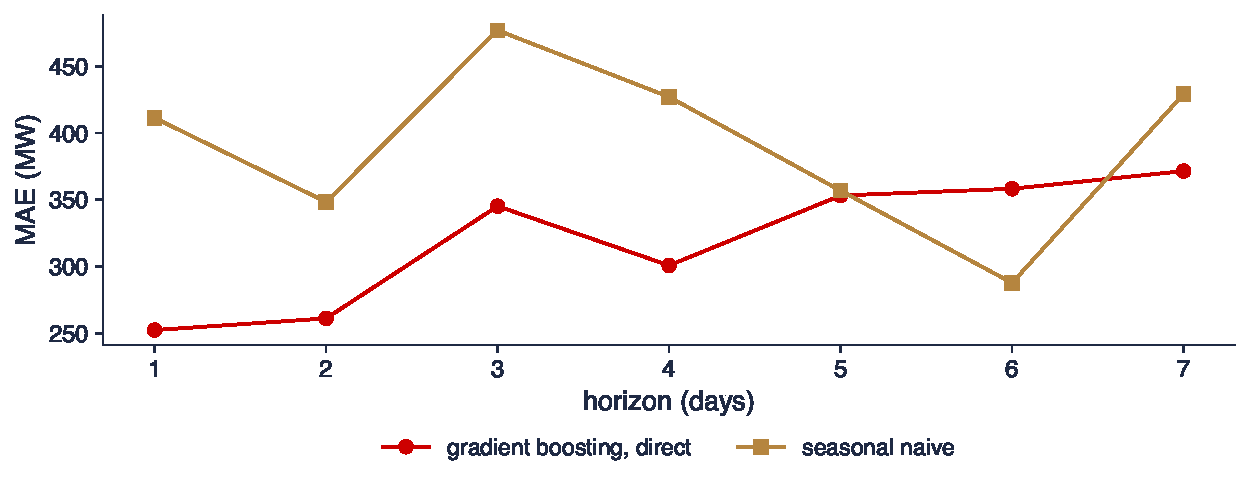
\includegraphics[width=0.96\textwidth,height=0.34\textheight,keepaspectratio]{ch9_sem_b1.pdf}
\end{center}
\vspace{-2mm}
\begin{itemize}
    \item 25 de origini, 7 orizonturi; MAE: GB 320 MW, naivă sezonieră 391 MW; RMSE 409 și 521 MW; MASE 1{,}04 și 1{,}27 (scala 308 MW)
    \item DM (cu corecția HLN) $= -2{,}63$, p 0{,}015; cea mai proastă origine pentru GB: 5 ianuarie 2026 (MAE 576 MW)
    \item Interpretare: cu o zi înainte, GB are 252 MW față de 411 MW: folosește nivelul de ieri, pe care metoda naivă sezonieră îl ignoră; la 7 zile (371 și 429 MW) ambele se bazează pe tiparul săptămînii trecute
\end{itemize}\quantlet{TSA\_ch9\_seminar}{\qlurl{TSA_ch9_seminar}}
\end{frame}

\begin{frame}{B2: recursiv, direct și valoarea sărbătorilor [Propus]}
\itemsize{\footnotesize}
\begin{itemize}
\item \textbf{Întrebarea}: prognozează strategia recursivă la fel de bine ca strategia directă și cît ajută variabilele de sărbătoare?
\item \textbf{Date}: datele și originile din B1; model: B1
\item \textbf{Cerințe}
\begin{enumerate}
    \item Repetați B1 cu strategia recursivă (\texttt{forecast\_recursive}).
    \item Repetați modelul direct fără cele trei variabile de sărbătoare (easter, xmas, holiday).
    \item Raportați MAE pentru cele trei modele pe toate zilele, pe zilele de sărbătoare legală și pe celelalte zile.
    \item Interpretare: ce grup de variabile explică cea mai mare parte a diferenței și în ce zile?
\end{enumerate}
\item \textbf{Raportați}: nouă valori MAE și o frază
\item Notebook: secțiunea B2
\end{itemize}
\end{frame}

\ifsolutions
\begin{frame}{B2: rezolvare [Propus]}
\itemsize{\scriptsize}
\begin{center}
\includegraphics[width=0.96\textwidth,height=0.34\textheight,keepaspectratio]{ch9_sem_b2.pdf}
\end{center}
\vspace{-2mm}
\begin{itemize}
    \item MAE (MW): direct 320, recursiv 327, direct fără sărbători 323
    \item În cele 9 zile de sărbătoare: 470, 409 și 496 MW; în celelalte zile: 312, 323 și 313 MW
    \item Interpretare: eliminarea indicatorilor de sărbătoare crește eroarea în zilele de sărbătoare (de la 470 la 496 MW) și lasă celelalte zile aproape neschimbate; sărbătorile rămîn cele mai grele zile pentru toate modelele; strategiile recursivă și directă diferă puțin
\end{itemize}\quantlet{TSA\_ch9\_seminar}{\qlurl{TSA_ch9_seminar}}
\end{frame}
\fi

\begin{frame}{B3: inflația din România cu trei luni înainte [Rezolvat]}
\itemsize{\footnotesize}
\begin{itemize}
\item \textbf{Întrebarea}: poate învățarea automată prognoza inflația din România cu trei luni înainte mai bine decît mersul aleator și un model AR liniar?
\item \textbf{Date}: inflația anuală IAPC a 27 de țări UE (Eurostat), lunar, 2005--2026
\item \textbf{Cerințe}
\begin{enumerate}
    \item Construiți variabilele fiecărei țări (decalajele inflației, variațiile lunare, luna calendaristică) și ținta $\pi_{t+3} - \pi_t$ cu \texttt{inflation\_frame}.
    \item În fiecare ianuarie din 2016, reestimați AR, lasso, random forest și GB doar pe România, precum și un GB global pe toate țările; prognozați fiecare lună a anului.
    \item Calculați RMSE pentru fiecare model și raportul lui față de mersul aleator.
    \item Aplicați testul DM pentru AR față de RW și pentru GB global față de GB local.
    \item Interpretare: ce s-a întîmplat cu toate modelele în 2021--2023?
\end{enumerate}
\item \textbf{Raportați}: șase valori RMSE, două teste DM și o frază
\item Notebook: secțiunea B3
\end{itemize}
\end{frame}

\begin{frame}{B3: rezolvare [Rezolvat]}
\itemsize{\scriptsize}
\begin{center}
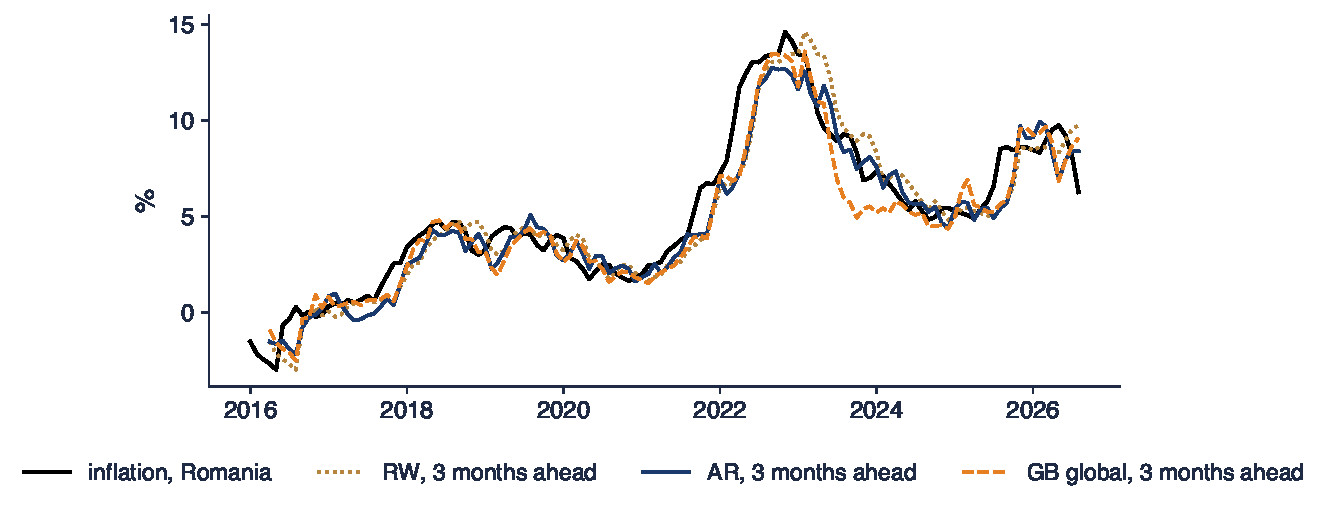
\includegraphics[width=0.96\textwidth,height=0.32\textheight,keepaspectratio]{ch9_sem_b3.pdf}
\end{center}
\vspace{-2mm}
\begin{itemize}
    \item 125 de origini, ianuarie 2016--mai 2026; RMSE (pp): RW 1{,}41, AR 1{,}28 (0{,}90), lasso 1{,}45 (1{,}02), RF 1{,}49 (1{,}06), GB local 1{,}64 (1{,}16), GB global 1{,}37 (0{,}97)
    \item DM: AR față de RW $-1{,}33$ (p 0{,}186); GB global față de GB local $-1{,}60$ (p 0{,}113)
    \item Interpretare: de la jumătatea lui 2021 pînă la jumătatea lui 2023, toate valorile RMSE cresc (RW 2{,}27, AR 2{,}02, GB global 2{,}09 pp): șocul energetic nu se afla în trecutul inflației; combinarea a 27 de țări ajută arborii, dar niciun model nu este semnificativ mai bun decît AR
\end{itemize}\quantlet{TSA\_ch9\_seminar}{\qlurl{TSA_ch9_seminar}}
\end{frame}

\begin{frame}{B4: semnul randamentelor BET [Propus]}
\itemsize{\footnotesize}
\begin{itemize}
\item \textbf{Întrebarea}: poate un clasificator prognoza dacă BET crește mîine mai bine decît „crește întotdeauna”?
\item \textbf{Date}: randamentele logaritmice zilnice ale BET din 2000; anii de test 2015--2026; model: B3 (reestimări anuale)
\item \textbf{Cerințe}
\begin{enumerate}
    \item Construiți variabilele din \texttt{sign\_frame} (cinci randamente întîrziate, sume pe 5, 21, 63 de zile, volatilitatea pe 21 și 63 de zile) și ținta $1\{r_{t+1} > 0\}$.
    \item În fiecare ianuarie, estimați o regresie logistică și un clasificator gradient boosting pe toate zilele anterioare; reperul prognozează clasa majoritară din datele de antrenare.
    \item Raportați acuratețea celor trei, statistica $z$ față de reper și AUC.
    \item Interpretare: ce spune rezultatul despre eficiența în formă slabă a pieței de la București?
\end{enumerate}
\item \textbf{Raportați}: trei valori ale acurateței, două statistici $z$, două valori AUC și o frază
\item Notebook: secțiunea B4
\end{itemize}
\end{frame}

\ifsolutions
\begin{frame}{B4: rezolvare [Propus]}
\itemsize{\scriptsize}
\begin{center}
\includegraphics[width=0.96\textwidth,height=0.32\textheight,keepaspectratio]{ch9_sem_b4.pdf}
\end{center}
\vspace{-2mm}
\begin{itemize}
    \item 2\,925 de zile de test; zile de creștere 55{,}3\%; acuratețea: reper 55{,}3\%, logit 54{,}7\% ($z = -0{,}63$, p 0{,}527), GB 52{,}9\% ($z = -2{,}64$, p 0{,}008)
    \item AUC: logit 0{,}538, GB 0{,}528; modelul logit prognozează „creștere” în 95{,}4\% din zile
    \item Interpretare: niciun cîștig față de reper; randamentele trecute nu conțin aproape nicio informație despre semnul următor, cum spune eficiența în formă slabă
\end{itemize}\quantlet{TSA\_ch9\_seminar}{\qlurl{TSA_ch9_seminar}}
\end{frame}
\fi


%=============================================================================
\section{Partea C: întrebări deschise și critica unui răspuns AI}
%=============================================================================

\begin{frame}{C1: un model global pentru consumul de energie din Europa [Propus]}
\itemsize{\footnotesize}
\begin{itemize}
    \item \textbf{Ideea}: ENTSO-E publică consumul orar al fiecărei țări europene; un model GB global antrenat pe 20 de țări poate prognoza România mai bine decît unul local
    \begin{itemize}
        \item variabile: decalaje scalate cu media fiecărei țări, ziua săptămînii, sărbătorile naționale, un identificator al țării
    \end{itemize}
    \item Întrebări la care trebuie să răspundeți
    \begin{itemize}
        \item 1. Depășește modelul global GB local și DHR pe cele 26 de origini din \tsachlink{https://danpele.github.io/Time-Series-Analysis/RO/Cursuri/capitol4_sezonalitate_prognoza.pdf}{Capitolul 4}?
        \item 2. Prognozează mai bine Paștele ortodox, deși majoritatea țărilor sărbătoresc Paștele occidental?
        \item 3. Ce țări ajută cel mai mult România (eliminînd pe rînd cîte o țară)?
    \end{itemize}
    \item Un posibil proiect de echipă: date, cod, teste DM și un raport de două pagini; model: B1, B3
\end{itemize}
\end{frame}

\begin{frame}{C2: verificați un răspuns AI [Propus]}
\itemsize{\scriptsize}
\begin{itemize}
    \item Un student a întrebat un asistent AI dacă învățarea automată poate prognoza piețele și consumul de energie. Răspunsul:
    \item \aiprompt{(a) Un random forest validat cu 5 grupuri explică 36{,}8\% din randamentul S\&P 500 din luna următoare, deci piața este previzibilă.}
    \item \aiprompt{(b) Un model logistic prognozează semnul zilnic cu acuratețea de 53{,}8\%, mult peste 50\%: un semnal profitabil.}
    \item \aiprompt{(c) Pentru consum, GB are MASE 0{,}97, deci este cu 3\% mai precis decît DHR.}
    \item \aiprompt{(d) Standardizați întîi toată seria, apoi împărțiți-o în antrenare și test.}
    \item \aiprompt{(e) Un LSTM bate întotdeauna ARIMA, pentru că are memorie lungă.}
    \item \aiprompt{(f) Variabilele de calendar ale zilei-țintă, precum sărbătorile, sînt permise, deoarece se cunosc dinainte.}
    \item Cerințe
    \begin{itemize}
        \item 1. Pentru fiecare afirmație, precizați dacă este corectă; dacă nu este, formulați afirmația corectă și, acolo unde se poate, dați valoarea corectă din notebook-ul cursului (secțiunile 2, 6, 9).
        \item 2. Raportați: o listă de șase verdicte, fiecare cu un rînd de justificare.
    \end{itemize}
\end{itemize}
\end{frame}

\ifsolutions
\begin{frame}{C2: rezolvare [Propus]}
\itemsize{\scriptsize}
\begin{itemize}
    \item (a) Greșit: țintele suprapuse pe 21 de zile se scurg între grupurile amestecate; walk-forward dă $R^2$ = -38{,}6\%
    \item (b) Greșit: reperul „întotdeauna în creștere” are 54{,}4\%; modelul este sub el
    \item (c) Greșit: MASE compară cu metoda naivă sezonieră în eșantion, nu cu DHR; DHR are MASE 0{,}89, deci GB este mai puțin precis decît DHR
    \item (d) Greșit: scurgere de informație; scalarea se estimează doar pe fiecare fereastră de antrenare
    \item (e) Greșit: pe datele noastre de consum, LSTM are MASE 1{,}16, mai slab decît DHR, GB și ridge; M4: metodele ML pure au pierdut în fața combinațiilor simple
    \item (f) Corect
\end{itemize}\quantlet{TSA\_ch9\_seminar}{\qlurl{TSA_ch9_seminar}}
\end{frame}
\fi


%=============================================================================
\section{Încheiere}
%=============================================================================

\begin{frame}{Idei de reținut}
\itemsize{\small}
\begin{itemize}
    \item O prognoză este o predicție din variabile cunoscute la origine: decalaje, medii mobile trecute, calendar
    \item Strategiile recursivă și directă: le comparăm pe aceleași origini
    \item Scurgerea de informație: orice valoare de după origine, inclusiv prin scalare sau prin grupuri amestecate
    \item GB depășește prognoza naivă sezonieră pentru consum; nimic nu depășește „întotdeauna în creștere” pentru semnul randamentelor BET
    \item Un răspuns AI este o ciornă: verificați schema de validare și reperul din spatele fiecărei acurateți declarate
\end{itemize}
\end{frame}

\begin{frame}{După seminar}
\itemsize{\small}
\begin{itemize}
    \item Cursul 9 dezvoltă fiecare temă de azi: variabile și strategii, validarea walk-forward, ridge și lasso, arbori și boosting, rețele neuronale și LSTM, intervale de prognoză, modele globale, competițiile M4 și M5
    \item Încercați cerințele [Propus] în notebook
    \item C1 poate deveni un proiect de echipă: un model global pentru consumul de energie din Europa
    \item Lectură: \refHP, cap.~10; \refFPP, secț.~12.4; \refMMH
    \item \textbf{Seminarul are rol de exercițiu și nu se notează; rezolvările cerințelor [Propus] se discută la seminar}
\end{itemize}
\end{frame}


%=============================================================================
\section{Bibliografie}
%=============================================================================

\begin{frame}{Bibliografie}
\itemsize{\tiny}
\begin{itemize}
    \item Diebold, F. X., \& Mariano, R. S. (1995). Comparing predictive accuracy. \textit{Journal of Business \& Economic Statistics}, 13(3), 253--263. \href{https://doi.org/10.1080/07350015.1995.10524599}{doi:10.1080/07350015.1995.10524599}
    \item Huang, C., \& Petukhina, A. (2022). \textit{Applied Time Series Analysis and Forecasting with Python}. Springer. \href{https://doi.org/10.1007/978-3-031-13584-2}{doi:10.1007/978-3-031-13584-2}
    \item Hyndman, R. J., \& Athanasopoulos, G. (2021). \textit{Forecasting: Principles and Practice} (3rd ed.), Section 12.4, Neural network models. OTexts. \href{https://otexts.com/fpp3/nnetar.html}{otexts.com/fpp3/nnetar.html}
    \item Hyndman, R. J., \& Koehler, A. B. (2006). Another look at measures of forecast accuracy. \textit{International Journal of Forecasting}, 22(4), 679--688. \href{https://doi.org/10.1016/j.ijforecast.2006.03.001}{doi:10.1016/j.ijforecast.2006.03.001}
    \item Kaufman, S., Rosset, S., Perlich, C., \& Stitelman, O. (2012). Leakage in data mining: Formulation, detection, and avoidance. \textit{ACM Transactions on Knowledge Discovery from Data}, 6(4), 1--21. \href{https://doi.org/10.1145/2382577.2382579}{doi:10.1145/2382577.2382579}
    \item Koenker, R., \& Bassett, G. (1978). Regression quantiles. \textit{Econometrica}, 46(1), 33--50. \href{https://doi.org/10.2307/1913643}{doi:10.2307/1913643}
    \item Lei, J., G'Sell, M., Rinaldo, A., Tibshirani, R. J., \& Wasserman, L. (2018). Distribution-free predictive inference for regression. \textit{Journal of the American Statistical Association}, 113(523), 1094--1111. \href{https://doi.org/10.1080/01621459.2017.1307116}{doi:10.1080/01621459.2017.1307116}
    \item Montero-Manso, P., \& Hyndman, R. J. (2021). Principles and algorithms for forecasting groups of time series: Locality and globality. \textit{International Journal of Forecasting}, 37(4), 1632--1653. \href{https://doi.org/10.1016/j.ijforecast.2021.03.004}{doi:10.1016/j.ijforecast.2021.03.004}
\end{itemize}
\end{frame}

\end{document}
